\documentclass[a4paper,twoside, openright,12pt]{report}
\usepackage{psfrag,amsbsy,graphics,float,amsmath,amssymb,epstopdf}
\usepackage{graphicx, color, mathtools} %deleted [dvips] in front of {graphicx, color} for usage with PDFLaTeX
\usepackage[latin1]{inputenc}
\usepackage{verbatim} 

%%% Stand 14.09.2007
%%% erstellt von Marion Sobotka
%%% marion.sobotka@tum.de
%%% last changes: 14.01.09


%_______Kopf- und Fußzeile_______________________________________________________
\usepackage{fancyhdr}
\pagestyle{fancy}
%um Kopf- und Fußzeile bei chapter-Seiten zu reaktivieren
\newcommand{\helv}{%
   \fontfamily{phv}\fontseries{a}\fontsize{9}{11}\selectfont}
\fancypagestyle{plain}{	
	\fancyfoot{}% keine Fußzeile
	\fancyhead[RE]{\helv\leftmark}% Rechts auf geraden Seiten=innen; in \leftmark stehen \chapters
	\fancyhead[LO]{\helv\rightmark}% Links auf ungeraden Seiten=außen;in \rightmark stehen \sections
	\fancyhead[RO,LE]{\thepage}}%Rechts auf ungeraden und links auf geraden Seiten
%Kopf- und Fußzeile für alle anderen Seiten
\fancyfoot{}
\fancyhead[RE]{\helv\leftmark}
\fancyhead[LO]{\helv\rightmark}%alt:\fancyhead[LO]{\itshape\rightmark}
\fancyhead[RO,LE]{\thepage}
%________________________________________________________________________________


%_Definieren der Ränder und Längen__________
\setlength{\textwidth}{15cm}
\setlength{\textheight}{22cm}
\setlength{\evensidemargin}{-2mm}
\setlength{\oddsidemargin}{11mm}
\setlength{\headwidth}{15cm}
\setlength{\topmargin}{10mm}
\setlength{\parindent}{0pt} % Kein Einrücken beim Absatz!!
%___________________________________________

%_Hyperref for CC Url__________
\usepackage{hyperref}
%___________________________________________

%_______Titelseite__________________________________________
\begin{document}
\pagestyle{empty}
\enlargethispage{4.5cm} %Damit das Titelbild weit genug unten ist!
\begin{center}
\phantom{u}
\vspace{0.5cm}
\Huge{\sc Control of a multi-robot cooperative team guided by a human-operator}\\
\vspace{1.5cm}
                                 \large{%eingereichte\\
			  %DIPLOMARBEIT\\%/STUDIENARBEIT/MASTERRBEIT/BACHELORARBEIT\\ 
                                           %von\\
                                 \large{Zwischenbericht zur\\
										MASTERARBEIT\\ 
										   von\\}          

						\vspace{0.4cm}
					cand. ing. Martin Angerer\\
						\vspace{0.5cm}
					geb. am 10.06.1991\\
					wohnhaft in:\\
					Steinheilstrasse 5\\
					80333 M\"unchen\\
					Tel.: 0151\,57978548\\
					\vspace{1.5cm}
					Lehrstuhl f\"ur\\
					INFORMATIONSTECHNISCHE REGELUNG \\
					Technische Universit\"at M\"unchen\\
					\vspace{0.6cm}
                    Univ.-Prof. Dr.-Ing. Sandra Hirche}
\end{center}
\vspace{5.0cm}
\begin{tabular}{ll}
Betreuer: Selma Musi\'c, M.Sc.  \\
Beginn: & 01.10.2015  \\
Zwischenbericht: &  11.01.2016  \\
Abgabe: &  01.04.2016 \\
\end{tabular}
%____________________________________________________________

\newpage
\cleardoublepage



\phantom{u}
\phantom{1}\vspace{6cm}
\begin{center}
In your final hardback copy, replace this page with the signed exercise sheet.
\end{center}

\newpage


%_______Abstract_____________________________________________
\topmargin5mm
\textheight220mm
\pagenumbering{arabic}
\phantom{u}
\begin{abstract}
  A short (1--3 paragraphs) summary of the work. Should state the problem, major assumptions, basic idea of solution, results. Avoid non--standard terms and acronyms. The abstract must be able to be read completely on its own, detached from any other work (e.g., in collections of paper abstracts). Don't use references in an abstract.
\begin{center}	
\normalsize \textbf{Zusammenfassung}\\
\end{center}
Hier die deutschsprachige Zusammenfassung
\end{abstract}
%____________________________________________________________

\newpage

%_______Widmung_______________________________________________
\phantom{u}
\phantom{1}\vspace{6cm}
\begin{center}
%Hier die Widmung oder leer lassen
\end{center}
%_____________________________________________________________



\pagestyle{fancy}

%_________Inhaltsverzeichnis__________________________
\tableofcontents 
%_____________________________________________________


%\chapter{Working with this Template}
%
%Make sure your thesis is well structured, that each major section does what it is supposed to do, and that the whole thing hangs together. The basic structure is often as given in this template (but other structures are possible). In particular, don't think you need to have exactly as many major sections or chapters as the list implies; sometimes it makes sense to merge things, sometimes it makes sense to move things (e.g., the literature review is in many papers deferred until after the results), sometimes it makes sense to split a logical part into several individual sections. Just use some common sense.
%
%Hand in your thesis at minimum \textbf{one week} before the deadline for correction. You will receive feedback for the final version and very likely have to do minor or major revisions of your writing. Plan your writing schedule to allow for these adjustments, which can have quite some impact on your grade! 
%
%\section{Style and Expressions}
%
%Before handing in your thesis, even for an intermediate review, please perform a spellcheck and correct grammar mistakes. The report is not meant to be a narrative text. Please stick to neutral and technical style and avoid subjective or biased expressions or adjectives/adverbs such as \emph{obviously, always, very, especially well, actually, so-called etc}. Scientific writing is about precision and you should underpin your statements factually, not soften them with unnecessary qualifiers.
%
%\subsection{Subsection}
%
%Use chapters, sections and subsections to structure your document
%
%\subsubsection{Subsubsection}
%
%Subsubsections can be used to further structure information within a subsection. They don't show up in your list of contents.
%
%\paragraph{Paragraphs} are sometimes more useful than subsubsections to structure text without breaking the flow.
%
%\section{Compiling}
%Linux: 
%do the following in a Shell:\\
%\begin{verbatim}
%latex myfile
%dvips myfile
%ps2pdf -sPAPERSIZE=a4 myfile.ps
%\end{verbatim}
%Make sure to use the A4 option, when you print the pdf!
%
%\section{Equations}
%Equations are written like that $x^2$. Or like that:
%\begin{equation}
%x^2
%\label{EQ:gleichung1}
%\end{equation}
%You can use (\ref{EQ:gleichung1}) to reference an equation in the
%text. Equations without reference number:
%\[
%x^2
%\]
%
%Please type all numbers in mathematics mode.
%Mathematical equations which are not part of the text should be centred.
%A parameter or variable must not be used at the beginning of a sentence.
%Type physical units as normal text, e.g. s, not $s$!
%Formulas must not jut out over the text margin, so take care to stay within the margins and eventually break the equation into several lines.
%Explain the variables you use. For each newly introduced variable, at least a short description of it should follow the equation in the style of \emph{\ldots with $x$ being the position of the cart and $u$ the control input.}
%In columns, align equations with the arithmetic operator \verb|(=,<, ...)|.
%Mathematical units must be consistently labeled with only one variable. Do not
%use a variable for more than one mathematical unit.
%
%\section{Figures}
%
%For pictures, it is convenient, if they are .eps.
%\begin{figure}[htb]
%\centering
%%\includegraphics[width=0.6\textwidth]{abbildung.eps}
%\caption[Abbreviated Description]{Long Description: The subtitles of tables and illustrations should be self-explanatory.}
%\label{FIG:abb1}
%\end{figure}
%
%Every illustration must be described and referenced in the text, cf. Fig. \ref{FIG:abb0}. 
%There is no such thing as a decorative figure! 
%If the figure is not mentioned in the text and therefore lacks an explanatory function, leave it.
%Lines in plots need to be clearly distinguishable, also in black-and-white print. 
%The subtitles and axis labels must be clearly legible (i.e. big enough) and include a scaling.
%If the illustration is copied from another person's work, you need to mention the
%source with \verb|\cite{}|.
%
%\section{Citations}
%
%For bibliography, edit {\tt mybib.bib} and list all
%references in a special style, e.g. for a book: 
%\begin{verbatim}
%@book{literaturselle1,
% author    = {S. Sastry},
% title     = {Nonlinear Systems - Analysis, Stability, and Control},
% publisher = {Springer},
% year      = 1999
%}
%\end{verbatim}
%
%Cite references in the text by.
%
%In order to have your references shown in your PDF, compile by:
%
%\begin{verbatim} 
%latex myfile
%bibtex myfile
%latex myfile
%latex  myfile
%dvips myfile
%ps2pdf -sPAPERSIZE=a4 myfile.ps
%\end{verbatim}
%
%Whether to use numeric or alphabetic references isn't all that important (unless prescribed by a conference or journal), but alphabetic tends to be more readable. Independent of citation style, the following rules should be followed:
%
%\begin{itemize}
%\item Use the \LaTeX~cite package. It doesn't give you additional commands, but it fixes a few quirks in \LaTeX. Among others it automatically sorts multiple citations, and it correctly spaces the angular brackets (if you use the \verb|\cite| command without leading white space).
%
%\item Citing several papers at one point should be done with a single \verb|\cite| command. For example, use \verb|gives good results\cite{Bloe_99, Jay_87}|, resulting in gives good results \cite{Bloe_99, Jay_87}. 
%
%Do not use \verb|gives good results\cite{Bloe_99}\cite{Jay_87}| which produces the ugly gives good results \cite{Bloe_99}\cite{Jay_87}. Also, note that there is no space between the \verb|\cite| command and the preceding word, \LaTeX~(with the cite package) does the spacing correctly.
%
%
%\item Avoid citations of the kind: \cite{Bloe_99} thinks that $x>y$ is valid, but \cite{ONeill_2000} argues that this is invalid in case of $z\geq5$. This works a bit better if using alphanumeric citation labels. Better, though, use the author's names: Bloe and Joe [1] think that $x>y$ is valid, but O'Neill et al. \cite{ONeill_2000} argues that this is invalid in case of $z\geq5$. 
%
%
%\item BibTeX is a great tool, but you need to know how to use it. A regular trap is to forget that \TeX~knows more about typesetting than you do. So, for example, it changes the case of words in the title. If your title contains acronyms and proper names (most do), they tend to get down-cased. Any such words which should not have their case changed should be put into braces, e.g., \verb|{The {Mungi} {OS} and its Use in Merry-Go-Round Seat Allocation}|.
%
%
%\item In citations don't abuse the category technical report. People tend to cite just about anything that hasn't been published in a journal or conferences as a TR. This is outright wrong. The concept of a TR is actually fairly well defined: A TR is published in some sort. This is generally as part of a formal TR series of some institution, in hardcopy or on the web or both. (They aren't always called "technical report", other common names are "research report", "technical memorandum", $<$institution$>$ "report" etc.) The publication (i.e. availability outside) is essential, otherwise it's at best an internal report.
%A TR has a number (absolutely!), an institution (publisher), a date (month and year at least) and a publisher's address (besides all the other stuff bibentries have).
%If your document doesn't have these features, it's not a TR. It's probably better categorized as a working paper. Even then it has a date and an institution address.
%
%\item Citing web pages is often unavoidable (but also often a sign of laziness). When citing web pages be aware that they may only be short-lived. Consider whether the reference will be of any use to the reader at all if the link is broken. Or whether your whole document only has a use-by date a few months past writing.
%
%\end{itemize}
%
%Any cited document, whatever it may be, has a few \textbf{mandatory} features:
%\begin{itemize}
%	\item Date. Absolutely. 
%	\item Author/organization/creator/person responsible for contents.
%	\item Whatever information the reader needs to find that document. In most BibTeX entry types these are clearly identified as mandatory fields. Mandatory means that they aren't optional. Don't pretend they are. For a working paper these might be the contact details of the author.
%\end{itemize}





%_________Einleitung__________________________________
\chapter{Introduction}

%\textit{Your first chapter in the document.
%Introduce the problem (gently!). Try to give the reader an appreciation of the difficulty, and an idea of how you will go about it. It's like the overture of an opera: it plays on all the relevant themes.}
%
%\textit{Make sure you clearly state the vision/aims of your work, what problem you are trying to solve, and why it is important. While the introduction is the part that is read first (ignoring title and abstract) it is usually best written last (when you actually know what you have really achieved). Remember, it's the first thing that is being read, and will have a major influence on the how the reader approaches your work. If you bore them now, you've most likely lost them already. If you make outrageous claims pretend to solve the world's problems, etc, you're likely fighting an uphill battle later on. Also, make sure you pick up any threads spun in the introduction later on, to ensure that the reader thinks they get what they have been promised. Don't create an expectation that you'll deliver more than you actually do. Remember, the reader may be your marker (of a thesis) or referee (of a paper), and you don't want to annoy them.} \\
%\\
Cooperative manipulation involves two or more robot arms collectively moving or manipulating a common object \cite{CoopManipHandbook}. Such a set-up overcomes many limitations seen by single robots. The prime example is the transportation of a large or heavy object, where a single manipulator would exert large local torques on the object. Back in the 1940s two remote manipulators were used to handle radioactive goods \cite{Goertz_52}. Around 1990 the \emph{NASA} researched cooperative manipulation in space construction applications \cite{Schneider_92}. Specifically in \cite{Lee_05} a cooperative manipulation strategy for the repair of the Hubble Space Telescope is proposed. Other tasks are for example:
\begin{itemize}
	\item assembly of multiple parts without using special fixtures
	\item grasping an object without rigid fixture but by exerting a suitable squeezing force
	\item deforming a flexible object
	\item coordinated use of tools
\end{itemize}
For the last point a recent application has been presented at the Fukushima Daiichi Nuclear Power Station. By equipping a two-armed robot with different tools it is capable of grasping an item (e.g. piping) and cutting it with the other, see Fig. \ref{FIG:MEISTeR}. For sensitive tools like an angle grinder it is favourable that movement and contact forces of both arms are coordinated.\\
\begin{figure}
	\centering
	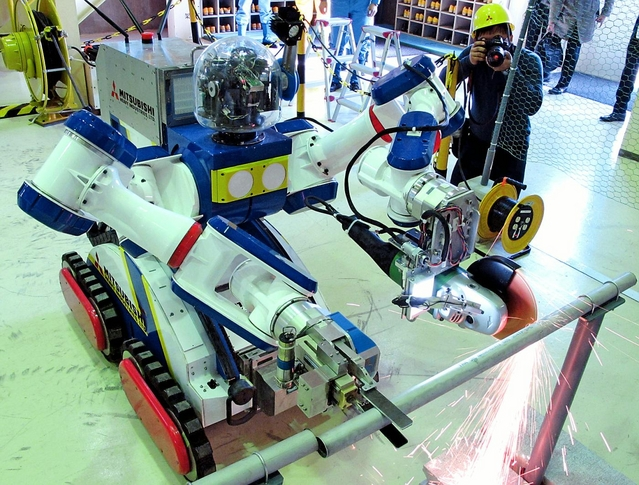
\includegraphics[width=0.8\textwidth]{mhi-meister.jpg}
	\caption[Demonstration of MHI MEISTeR at Fukushima Daiichi NPS]{Demonstration of the tele-operated MHI MEISTeR robot at Fukushima Daiichi Nuclear Power Station}
	\label{FIG:MEISTeR}
\end{figure}
Space and hazardous environments are fruitful environments for cooperative manipulators, often they are directly controlled by a human operator. Combining human reasoning and the enhanced flexibility of a cooperative set-up is a powerful combination in an unstructured environment. A human in the control loop comes with superior foresight and planning capabilities. Therefore different control architectures exist, which can be classified by the level of autonomy of the robot system. In an direct master-slave approach each robot is controlled independently by a human operator. This is impractical due to formation requirements. Lee \cite{Lee_05} treats the constrained system as a single slave, while the formation is preserved by the robots autonomously. Many master-slave systems give the operator force-feedback, while she/he commands the motion. This helps the operator compensate for resistances and gives a natural feeling of the interaction with the environment. The structure then is fully bi-directional, ones refers to bilateral telemanipulation. The human is part of the closed loop, since her/his behaviour is directly influenced by the experienced force-feedback. For a remotely located set-up, the time delays in communication may lead to undesired motions, stability of the human-in-the-loop system becomes an issue. Tactile or visual feedback eases this problem, since they are non-reactive. This means they do not induce operator movements reacting to a back-driving force \cite{Massimino_93}. A control architectures that leaves further autonomy to the robot system is Supervisory control, described by a closed local, autonomous control loop. It interacts with the operator by continuously sending information about the state and periodically receiving commands \cite{Sheridian_92}.\\

However a difficulty is the control of the set-up which possess extra degrees-of-freedom. There must be an intuitive way to control the formation of robots. The control scheme shapes each robot's motion to commit to the common task. A disadvantage of having a remotely located operator is an inevitable delay in the control loop. This restricts the operators possibilities to react to unexpected situations.\\

The major challenge in cooperative manipulation is to simultaneously control the forces between the manipulators and the object, so to say the internal stress exerted on the object, and the forces between the object and the environment, i.e. the absolute motion of the object.
Strategies that map force and velocity of the object to the manipulators have to be considered.\\
One important assumption is the nature of the connection between manipulator and object. It can be seen as rigid or more general as friction-based. With a rigid fixture the grasp is always stable, on the contrary friction grasps need to be actively stabilized. To comply with the friction constraints a contact normal force has to be set, dependent on the tangential components present during manipulation.\\
Towards a versatile usage of cooperative manipulation it is vital to let the human operator control the robotic system intuitively and naturally. 
A promising approach is gesture control. Gioioso et al. \cite{Gioioso_2014} demonstrated this for a formation of unmanned aerial vehicles. They are able to control opening and closing of the grasp. In a grasped state the objects's pose and the grasping forces can be changed, just by tracking gesture of a single human hand. 
Directly integrating the human into the control scheme makes use of the visual tracking capacities of the human and eases operation in unknown environments. Regardless of the operator being present on-site with the robots or not, hand tracking and analysis requires a certain time. This delay in the control loop can cause instability. The problem can be modelled as a transmission line with delay and treated with methods known from tele-operation.
The human takes the role of a supervisor, representing a high-level part of the control scheme. He is responsible for planning, choosing a trajectory and if necessary setting of grasping forces.
On a local low-level robots need to coordinate their motion compliant with the commanded trajectory and adjust their formation to realize the desired internal forces. For non-rigid fixtures the local robot controller requires the position of the other manipulators. The local communication between the robots causes delay, which has to be treated with tele-operation techniques in order to ensure stability.\\
Haptic feedback??

 

\section{Problem Statement}

%\textit{You can either state the problem you are trying to solve in the general introduction, providing the transition from the overall picture to your specific approach, or state it in a separate section. Even if you don't use the separate section, writing down in a few sentences why the problem you are trying to solve is actually hard and hasn't been solved before can give you a better idea of how to approach the topic. This can be also merged with the related work part.}\\

Manipulating an unknown object in an unstructured environment is an interesting task for a human-guided cooperative manipulation set-up. Dropping the assumption of a rigid- connection between manipulator and object, the grasp has to be actively stabilized under varying circumstances. During dynamic manipulation a slipping of contact due to the inertia of the object has to be avoided using an automatic mechanism. On the other hand the operator must directly adjust grasp forces for heavy or fragile objects.\\
Position and velocity of the manipulated object are difficult to track in an everyday setting. Usually only end-effector position and velocity of the robots are available. Object position has to be estimated from the known data.\\
For grasping an  object of unknown or even flexible shape, the determination of a fixed grasp map in advance is not useful. Size and shape of the grasp have to be determined by the operator during the grasp process. The controller has to be flexible to varying grasp geometries during the whole task execution.\\
Integrating the human into the control loop, energetic passivity of the closed loop system is a meaningful and intuitive way to ensure stability and a natural way of interaction. Energetic passivity limits the extractable mechanical energy from the closed loop system. This means that the potential damage is also limited. 
Energetic passivity of the robotic system ensures stability of the interconnection stability with any passive systems. Since humans and many relevant environments are passive the closed loop system will always be stable if the overall control scheme is designed energetically passive.


\section{Related Work}
Control strategies suitable for Cooperative Manipulation can be classified dependent on the nature of the manipulator-object connection: rigid-fixture and friction-grasps.
An import group within the former are the hybrid position/force control approaches. 
Control action is decomposed in a motion control loop, accounting for the tracking if the desired trajectory for the overall system and a force control loop to control the internal forces on the object. A pre-defined selection matrix determines for every workspace coordinate whether it is position or force controlled. Controlling the robot on joint level, the necessary torques can be computed using a PD plus gravity compensation control scheme. The desired joint positions and velocities are computed by inverse kinematics \cite{Wen_92}.
Object level control architectures often use feedback linearisation of the non-linear manipulator dynamics to achieve a linear and decoupled control of motion and grasping force \cite{Hsu_93}.
Force control is only meaningful if contact between manipulator and object. Motion control leads to unbounded forces if the motion direction is not consistent with the constraints,  since force in this direction is not controlled. The transition between contact and no contact during grasping cannot be handled with these approaches. For these reasons in the following only the better suited impedance control schemes are considered. Impedance control, introduced by Hogan \cite{Hogan_84}, is a well known strategy to avoid unbounded forces when it comes to interaction of manipulators with objects/environment. It does not control one state variable (position, velocity, force) dynamically enforces a relation between forces and system state. Contact directions do not have to be pre-specified. The controller is stable independently of the contact state.
A physical analogy the impedance control scheme is a spring-mass-damper system.\\  

%\textit{From Kevin Elphinstone's \emph{A Small Guide to Writing Your Thesis}\cite{Elphinstone2014}:}
%
%\textit{"The related work section (sometimes called literature review) is just that, a review of work related to the problem you are attempting to solve. It should identify and evaluate past approaches to the problem. It should also identify similar solutions to yours that have been applied to other problems not necessarily directly related to the one your solving. Reviewing the successes or limitations of your proposed solution in other contexts provides important understanding that should result in avoiding past mistakes, taking advantage of previous successes, and most importantly, potentially improving your solution or the technique in general when applied in your context and others.}

%\textit{In addition to the obvious purpose indicated, the related work section also can serve to:}

%\begin{itemize}
%	\item \textit{justify that the problem exists by example and} argument
%	\item \textit{motivate interest in your work by demonstrating relevance and importance}
%	\item \textit{identify the important issues}
%	\item \textit{provide background to your solution}
%\end{itemize}

%\textit{Any remaining doubts over the existence, justification, motivation, or relevance of your thesis topic or problem at the end of the introduction should be gone by the end of related work section.}

%\textit{Note that a literature review is just that, a review. It is not a list of papers and a description of their contents! A literature review should critique, categorize, evaluate, and summarize work related to your thesis. Related work is also not a brain dump of everything you know in the field. You are not writing a textbook; only include information directly related to your topic, problem, or solution."}

%\textit{Note: Do the literature review at an early stage of your project to build on the knowledge of others, not reinvent the wheel over and over again! There is nothing more frustrating after weeks or months of hard work to find that your great solution has been published 5 years ago and is considered old news or that there is a method known that produces superior results.}

\subsection{Control schemes for rigidly connected manipulators}\label{SS:rigidcontrolschemes}
A rigid fixture between manipulator and object means that both forces and moments are exchanged at the grasp points: all translational and rotational motion components can be transmitted through the contact points. The rigid connections are expressed by a number of kinematic constraints, which reduce the Degrees-of-Freedom (DoF) of the constrained system. The attempt to move in the constrained directions results in internal loading of the object. Therefore trajectories of the manipulators have to be generated to avoid internal stress on the object. Assuming a rigid connection normally no grasping force is needed to stabilize the grasp, i.e. internal forces are undesired because possibly harmful to the object. Nevertheless some papers propose possibilities to specify or control internal forces.\\
Among the first to use impedance control in cooperative manipulation were Schneider and Cannon \cite{Schneider_92}. They replaced the actual object by a virtual mass and connected it to the environment with a spring and a parallel damper. The resulting impedance equation is:
\begin{equation}
M_{o,d} (\ddot{x}_o^d - \ddot{x}_o) + D_o (\dot{x}_o^d - \dot{x}_o) + K_o(x_o^d,x_o) = h_{env} 
\end{equation}
Here $ M_{o,d} $ denotes the inertia of the virtual object, $ D_o $ is the damping along the spring, which is represented by $ K_o(x_d,x) $. $ x_o = (p_o^T,Q_o^T)^T $ is the stacked vector of position and orientation of the object. $ x^d $ denotes a desired quantity. The external wrench, exerted by the environment on the object, $ h_{env} = (f_{env}^T,t_{env}^T)^T$ consists of force and torque vectors.
The dynamics of the virtual object is then given as:
\begin{equation}
M_{o,d}\ddot{x} = -h_{env} + h_o^{\Sigma} = -h_{env} + M_{o,d}\ddot{x}_d + D_o (\dot{x}_d - \dot{x}) + K_o(x_d,x)
\end{equation}
The resulting impedance control output $ h_o^{\Sigma} $ is than mapped to the manipulators using a generalized inverse of the grasp matrix:
\begin{equation}
h^{\Sigma} = G^\dagger h_o^{\Sigma}
\end{equation}
Performance of this strategy depends on choosing the virtual inertia close to the actual, i.e. good knowledge of the object is required. Furthermore gravity compensation would be necessary to model the full object dynamics. In general the equation of motion for a rigid object is:
\begin{equation}\label{EQ:ObjectDynamics}
M_o \ddot{x}_o + C_o \dot{x}_o + g_o = h_{env} + h^\Sigma
\end{equation}
Wherein $ M_o $ is the actual object inertia, $ C_o $ is the Matrix accounting for the Coriolis force and $ g_o $ is the gravity. 
For notational convenience the pose dependencies of the parameter matrices, e.g. $ M_o(x_o) $, are omitted.\\
Bonitz and Hsia \cite{Bonitz_96} propose to model each manipulator as an impedance relation. Thereby a relation between manipulator dynamics and internal forces on the object is enforced:
\begin{equation}
M_i(\ddot{x}_i^d - \ddot{x}_i) + D_i (\dot{x}_i^d - \dot{x}_i) + K_i(x_i^d,x_i) = h_{int}
\end{equation}
$ M_i, D_i, K_i(x_i^d,x_i) $ are the desired inertia, damping and stiffness representations of the i-th manipulator.The internal wrench $ h_{int} = VV^\dagger h $ is calculated from the measured contact wrench $ h $. $ V $ is a basis of the nullspace of the grasp matrix, $ V^\dagger $ denotes the pseudoinverse. No assumptions on the object are necessary because it is not considered in the control scheme.\\ 
The first approach ensures compliant object-environment interaction, while the second limits internal forces even in case of end-effector displacements. The both have been combined by Caccavale and Villani \cite{Caccavale_01}. Their control architecture is cascaded, consisting of a two level reference trajectory generation and a motion control loop below. On top-level an impedance relation between object and environment is used to generate a compliant trajectory subject to environmental forces:
\begin{equation}
\alpha M_o(\ddot{x}_o^d - \ddot{x}_o^r)  + D_o(\dot{x}_o^d - \dot{x}_o^r) + K_o(x_o^d,x_o^r)  = h_{env}
\end{equation}
The constant $ \alpha $ scales the object inertia proportionally to a desired value.
The control output is the reference object acceleration $ \ddot{x}_o^r $, $ h_{env} $ is an input. This is sometimes called admittance control, admittance being the inverse of impedance. $ h_{env} $ has to be known, but is not easily measured in a practical set-up. Recalling (\ref{EQ:ObjectDynamics}) the environmental forces can be expressed as:
\begin{equation}
h_{env} =  M_o \ddot{x}_o^r + C_o \dot{x}_o^r + g_o - G^\dagger h
\end{equation}
Herein $ G^\dagger $ is a generalized inverse of the grasp matrix, selecting the motion inducing components from the measured contact wrench $ h $. $ \dot{x}_o^r, x_o^r $ are calculated from $ \ddot{x}_o^r $ by integration.
From the compliant object trajectory ($ \ddot{x}_o^r,\dot{x}_o^r,x_o^r $) the desired trajectories of the manipulator ($ \ddot{x}_i^d,\dot{x}_i^d,x_i^d $) using the kinematic constraints. The reference manipulator trajectory, enforcing compliant behaviour between manipulators and object, is calculated from manipulator dynamics and internal forces: 
\begin{equation}
M_i(\ddot{x}_i^d - \ddot{x}_i^r) + D_i (\dot{x}_i^d - \dot{x}_i^r) + K_i(x_i^d,x_i^r) = VV^\dagger h
\end{equation}
The control output is the reference acceleration of the i-th manipulator $ \ddot{x}_i^r $, $ \dot{x}_i^r,x_i^r $ are obtained from integration. These variables are the inputs the inner motion control loop (PD-type). The strategy of compliant trajectories allows for high gains in the motion controller. Knowledge of object dynamics and measurement of the contact wrenches is required.\\
In a frequently cited follow-up paper Caccavale et al. \cite{Caccavale_08} combine the concept of \emph{geometrically consistent stiffness} with the same architecture. This allows for selective stiffness behaviour along different directions.\\
Recently Heck et al. \cite{Heck_13} worked with this architecture, they assume knowledge of the environment instead of the object.
The environmental wrench is than derived as:
\begin{equation}
h_{env} =  \Sigma D_{env} (\dot{x}_o^d - \dot{x}_o^r)  + \Sigma K_{env}(x_o^d,x_o^r)
\end{equation}
It is assumed here that the environment has a constant stiffness and damping ($ K_{env}(x_o^d,x_o^r),D_{env}) $. $ \Sigma $ is a diagonal selection matrix modelling the direction of contact.\\
A combination of impedance control on manipulator/object level and feed-forward object dynamics is presented in\cite{DePascali_15}. The manipulators are modelled as springs and dampers, inertia is used to feed-forward the desired acceleration: 
\begin{equation}
M_i \ddot{x}_i^d + D_i (\dot{x}_i^d - \dot{x}_i) + K_i(x_i^d,x_i) = h^x
\end{equation}
This avoids the necessity of either measuring manipulator acceleration or contact force.
Object dynamics is represented with feed-forward term, mapped to the manipulators with a weighted pseudoinverse $ G^+ $ of the grasp matrix:
\begin{equation}
h^d = G^+ (M_o \ddot{x_o^d} + C_o \dot{x_o^d} + g_o)
\end{equation}
Note that this term is not an impedance relation and does not adjust if the environment hinders motion.
The combined control law is $ h^\Sigma = h^x + h^d $.\\
 


\subsection{Friction grasps in Cooperative Manipulation}
The assumption of rigid-fixture between object and manipulators only holds f the manipulators are equipped with  appropriate grasping devices. In analogy to a human this device would be fingers wrapping around an inhomogeneity on the object, to achieve a rigid grasp. For an even object (e.g. a ball) humans use their hand palms to realize a friction grasp. Grasp stability is ensured by pressing the object. Technical applications where cooperative manipulators should be able to do a friction grasp are numerous, e.g. when no appropriate grasping device is available (or shall be avoided) or the object structure is not graspable.\\
Research of friction grasps is mainly done with robotic hands, the fingertips being the contact points. Depending on the nature of the tip a certain number of contacts is required to achieve a firm grasp: for non-deformable and small but frictional contacts, three are required to hold an object with 6 \emph{DoF} tightly. This contact model is called \emph{Hard Finger} or \emph{Point Contact with Friction (PCwF)}. It allows to transmit forces along the contact normal in pushing direction and for forces in tangential plane. If the contact is deformable or of considerable size, two are sufficient contact points form a firm grasp. This is called \emph{Soft Finger} model. In addition to the \emph{Hard Finger} torques around the contact normal are transferred.\\
The problem of grasping divides into three sub-problems: selection of suitable grasp points, coordinated motion of the constrained system and control of the grasping force especially when interacting with the environment. The problem of coordinated motion is very similar to the case of rigid-fixture, while the control is exclusive to friction grasps. With robot hands it is most important to maintain a stable grasp. Undesired or unnecessary and possibly harmful internal forces occur during dynamic manipulation and interaction with the environment. Since discrete robots in cooperative manipulation are often powerful, proper control of the internal forces becomes more important.\\
For the reasons stated in the previous subsection hybrid position/force control approaches are less suitable than impedance control and will not be considered. The control architectures for rigid-fixture can be re-used if a internal force is applied in addition. By definition internal forces do not contribute to the motion of the constrained system and thus do not interfere with the control goals of rigid-fixture. Formally this can be described as $ G h_{int} = 0 $, i.e. the internal forces $ h_{int} $ lie in the null-space of the grasp matrix $ G $. To calculate desired internal forces a suitable vector $ z $ is multiplied with a basis of the null-space of the grasp matrix $ V $: $ h_{int}^d = V z $.\\
When it comes to position uncertainties of contact points or deformable objects, calculating internal forces from a fixed grasp matrix may lead to undesired results. One alternative are \emph{Artificial Potential Fields (AFP)} to realize a desired formation of manipulators relative to each other in 3D space. 
Sieber et al.\cite{Sieber_15} use \emph{AFP} to build up a formation of robots around an object. The object is grasped by varying the desired distances between the manipulators. The internal forces can thus be set in a physically meaningful way. The generated force of manipulator $ i $ in Cartesian direction $ k $ due to the springs connecting to the other manipulators $ j \in N_i $ is:
\begin{equation}
f_{i,k}^d = - \sum_{\substack{j\in N_i}} k_{ij} \dfrac{p_{i,k} - p_{j,k}}{\vert p_{i,k} - p_{j,k} \vert} (\vert p_{i,k}-p_{j,k}\vert - d_{ij,k})
\end{equation}
Notably here $ p\in\mathbb{R}^3 $ only represents the position of the manipulator, orientation information is omitted. Using the \emph{Hard Finger} contact model a pure translational representation is sufficient since it does not transmit torques. $ k_{ij} > 0$ is a control gain. The desired distance is defined by $ d_{ij,k} $.
The approach controls only the formation of the robots and does not take the object dynamics into account. Positional control for the object is done assuming the object to be in the middle of the manipulators: $ p_o = \frac{1}{N} \sum\nolimits_{i=1}^{N} x_i $. This has important advantages: no need to know the object's dynamics and no need for tracking the object.\\
Similar to the concept of \emph{AFP} are 1-\emph{DoF} springs with a desired rest-length. They only allow to set the absolute distance between two points in space, while \emph{AFP} control the distance along each direction. 1-\emph{DoF} can be more intuitive to control, because only one distance parameter has to be changed in contrast to a relative formation in 3D space.\\
One approach using 1-\emph{DoF} springs is the \emph{Static IPC} by Wimb\"ock et al. \cite{Wimboeck_06}. The concept of the \emph{intrisically passive controller (IPC)} was introduced by Stramigioli \cite{Stramigioli_01} and will be covered later on. Here the rest-length springs connect to the middle of the manipulator set-up. The force generated by a single spring connecting from manipulator $ i $ to the center is: $ k_{i} \frac{p_i - p_o}{\vert p_i - p_o \vert} (\vert p_i-p_o\vert - d_{i}) $. Here $ k_i \in \mathbb{R}^3 $ is the stiffness matrix and $ d_i $ is the rest-length of the $ i $-th spring.
Considering the cross-coupling of the springs the generated forces are:
\begin{equation}
f^d  = - \sum_{i=1}^N\left[\dfrac{\partial (p_i-p_o)^T}{\partial p} k_i \dfrac{p_i-p_o}{\vert p_i-p_o\vert}  (\vert p_i-p_o\vert - d_i) \right]
\end{equation}
Wherein $ \frac{\partial (p_i-p_o)^T}{\partial p} \in \mathbb{R}^{3N \times 3} $ is the cross-coupling matrix.
Furthermore this approach uses another spring to connect environment and object. This is a 6-\emph{DoF} spring, thus the object's position and orientation is controlled. Force and torque are computed as:
\begin{subequations}
\begin{align}
f_o^d = K_{o,t} R_o^T (p_o-p_o^d) \\
t_o^d = 4 J^T_{\omega\epsilon} K_{o,r} \epsilon_d 
\end{align}
\end{subequations}
The translational and rotational stiffness matrices are denoted by $ K_{o,t},K_{o,r} $. $ R_o $ is a rotation matrix indicating the object orientation, it is defined by the manipulator positions. $ \epsilon_d $ is the rotational error represented by the vector part of the quaternion, $ J^T_{\omega\epsilon} $ denotes the reduced quaternion product.\\
Damping along each spring is proposed. This important especially for the cross-coupling springs to suppress oscillatory internal motions.\\
While $ f^d $ acts on the manipulators, $ f_o^d $ and $ t_o^d $ act on the object. This is resolved by the hand geometry, different hand \emph{Jacobian} matrices cast the wrenches into joint torques. If no kinematic structure is present (e.g. when using discrete robots) often a weighted pseudoinverse of the grasp matrix (\cite{Schneider_92,DePascali_15}) is used. According to Stramigioli\cite{Stramigioli_01} the physically meaning of the weighting coefficients is small. Erhart and Hirche\cite{Erhart_15} recently presented weighted pseudoinverses based on inertia and geometry of object and manipulators. However (in some cases) this requires konwledge of the object properties. Stramigioli therefore introduces a virtual object, the wrench acts directly onto the virtual object and thus  influences its dynamics. The manipulators are connected to the virtual object with rest-length springs, so the object wrench is mapped to the manipulators via the virtual object dynamics.
Wimb\"ock et al. implement Stramigioli's \emph{IPC} in a simplified version on a four fingered robotic hand\cite{Wimboeck_08}. The dynamics of the virtual object are:
\begin{equation}
M_v \ddot{x}_v + C_v \dot{x}_v + g_v = w_v
\end{equation}
The virtual object wrench $ w_v $ is composed of environment interaction $ w_{vo} $ and manipulator forces $ f_c $: $ w_v = w_{vo} + G_v f_c $. Where $ G_v $ is the virtual grasp matrix. Environment interaction is described by a 6 \emph{DoF} spring: $ w_{vo} = K(x_v^d,x_v) $. The springs connecting to the manipulators exert the wrench on the virtual object: $ G_v f_c = G_v K_c (p - G_v^T x_v) $. The control law for the manipulators is already given as:
\begin{equation}
f = -f_c = K_c(G_v^T x_v - p)
\end{equation}
The stiffness matrix $ K_c = blockdiag(k_1 I_3, ... , k_n I_3)$ is isotropic. The rest-lengths of the springs are chosen by the size of the virtual object, i.e. by specifying the virtual grasp matrix $ G_v $.\\
One assumption in \cite{Wimboeck_08} is that internal forces are sufficient to ensure a firm grasp. This is done in a physically meaningful way by choosing the rest-lengths.
%Allowing a human to directly control the formation (e.g. with gestures), three parameters are to be specified by the operator: position, orientation and grasping force. Tracking and processing human inputs causes a delay, which can be compared to a telemanipulation setting, although the operator may be on-site. A local controller is required to ensure a secure grasp while human interfacing can be higher level control.

\subsection{Determination of desired internal forces}
Non-rigid grasps object and manipulators are connected with friction constraints. Contact force towards the object generates frictional force opposed to external forces tangential to the contact point. If the tangential forces exceed the frictional force the friction constraint is violated and contact slippage occurs. Squeezing or internal forces do not contribute to the motion of the constrained system. They need to be chosen sufficiently high to maintain a stable grasp under external forces acting on the object. On the other hand they must be bounded to not damage the object. These opposed requirements can be formulated as a cost function.\\
Buss et al. \cite{Buss_96} propose a cost function consisting of two factors: one is a barrier function tending to infinity for violating the friction constraint limit, the other is linear function rising with the exerted force, making high forces costly. The optimal desired internal force is the minimum of the cost function, thus the forces are chosen as small as possible, preserving a stale grasp.\\
Non-linear friction constraints are given for the \textit{point contact friction} and the \textit{soft contact friction} model:\\
The \textit{point contact friction} constraint allows transmitting force in tangential  and normal  (only towards the object) direction. In addition the \textit{soft contact} constraint transmits the torsional moment around the normal axes. Buss' main contribution is that friction constraints can be reformulated  equivalent to positive definite matrices. These matrices are used to construct the cost function. This results in a convex optimization problem, thus an optimum is always a global optimum. \\
Bicchi et al. \cite{Bicchi_98} limit their contribution to the \textit{point contact friction} model but expand the cost function. A maximum contact force is introduced, this is useful for rather loosing contact than destroying the object. Furthermore a minimum force in normal direction is specified to ensure grasp stability even under uncertainties. This two add up to with the friction constraint to a function, which has a negative scalar value if the set of constraints are respected. The sum of this functions for all contact points forms the cost function.\\ 
Han et al. \cite{Han_2000} reformulated Buss' positive definite matrix approach as a \textit{linear matrix inequality}(LMI) problem. Being a common optimization task, efficient solvers (e.g. interior point algorithm) exist. Calculation time could be significantly reduced.
%____________________________________________________



%_____Kapitel 2_________________________________
\chapter{Main Part}
%The controller is divided into two parts, the local one does the real-time interaction of the manipulators with the object. This part is passive, i.e. the robot along with its local controller has a certain amount of energy, the energy can not increase as long as no power is provided by the environment or the higher-level control part. Therefore the two parts will be called Intrinsically Passive Controller and Supervisor, this scheme was introduced by Stramigioli \cite{Stramigioli_01} as a general framework with application to robotic hands.
\section{port-Hamiltonian systems}
Port-Hamiltonian systems(PHS) provide a framework to for the geometric description of complex physical systems. The goal is divide the system in simple Hamiltonian subsystems and interconnect them using methods of network theory.\\
The Hamiltonian equations of motion are related to the better known Euler-Lagrange equations with the Legendre transformation. Both are formulations on energy level thus they are useful for a continuous description of mixed-energy systems, e.g. a pendulum alternating between kinetic and potential energy periodically.

\subsection{Hamiltonian description of mechanical systems}\label{SS:HSdescription}
The classical Hamiltonian equations for a mechanical system are:
\begin{eqnarray}
	\dot{q} = \frac{\partial H}{\partial p}(q,p)\\
	\dot{p} = -\frac{\partial H}{\partial q}(q,p) + F
\end{eqnarray}
Where Hamiltonian $ H(q,p) $ is the total energy of the system, $ q = (q_1,...,q_k)^T $ denotes the generalized coordinates of the system with $ k $-degrees of freedom and $ p = (p_1,...,p_k)^T $ is the vector of the generalized momenta. $ F $ is the input of generalized forces.\\
An important aspect of PHS is conservation of energy, i.e. supplied work is either stored in the system \cite{vanderSchaft_06}. The energy balance of the system is:
\begin{equation}
	\frac{d}{dt}H = \frac{\partial^T H}{\partial q}(q,p)\dot{q} + \frac{\partial^T H}{\partial p}(q,p)\dot{p} = \frac{\partial^T H}{\partial p}(q,p)F = \dot{q}^T F
\end{equation}
While the generalized force $ F $ is the input of the system, the output can be defined as $ e = \dot{q} $, for a mechanical system $ \dot{q} $ is the generalized velocity. Note that the product of Force and velocity is mechanical power.\\
PHS can be described in local coordinates $ x $ on the $ n $-dimensional state space manifold $ \mathcal{X} $, $ x \in \mathcal{X} $:
\begin{eqnarray}
	\dot{x} = J(x) \frac{\partial H}{\partial x}(x) + g(x)f \\
	e = g^T(x) \frac{\partial H}{\partial x}(x)
\end{eqnarray}
Where $ J(x) $ is the $ n \times n $ structure matrix, $ J(x) $ is skew-symmetric, i.e. $ J^T(x) = - J(x) $. Furthermore $g(x) $ is the $ n \times m $ input matrix and $ f \in \mathbb{R}^m $ is a general input vector. With the skew-symmetry of $J(x)$ the energy balance of the local coordinate system is $ \frac{dH}{dt}(x) = e^Tf $. \\
Any energy conservative physical element can be described in this formulation. To account for dissipative elements the previous can be extended by a positive semi-definite matrix $R(x)$.
\begin{eqnarray}
	\dot{x} = (J(x)-R(x)) \frac{\partial H}{\partial x}(x) + g(x)f \\
	e = g^T(x) \frac{\partial H}{\partial x}(x)
\end{eqnarray}
The energy balance changes since the supplied power is not only stored but dissipated:
\begin{equation}
	\frac{dH}{dt}(x) = e^Tf - \left( \frac{\partial H}{\partial x}(x) \right)^T R(x) \frac{\partial H}{\partial x}(x)
\end{equation}\\
Consider the example of a simple one-dimensional spring-mass-damper system described by $ M\ddot{x} = -kx -Dx +F $. Where $ M,k,D,F $ denote the mass, stiffness, damping and external force acting on the mass respectively.
In the usual state space formulation this is:
\begin{equation}
	\begin{bmatrix}\dot{x} \\ \ddot{x}\end{bmatrix} =
	\begin{bmatrix}0 & 1 \\ -\frac{k}{M} & -D\end{bmatrix}
	\begin{bmatrix}x \\ \dot{x}\end{bmatrix} + 
	\begin{bmatrix}0 \\ 1\end{bmatrix}F
\end{equation}
One obtains an alternative representation by choosing energy variables as state variables, i.e. the energy stored in the spring is described by the displacement $ x $ and the energy of the moving mass by the momentum $ p = M\dot{x} $:
\begin{equation}
	\underbrace{\begin{bmatrix}\dot{x} \\ \dot{p}\end{bmatrix}}_{\dot{\chi}} =
	\underbrace{\begin{bmatrix}0 & 1 \\ -1 & -D\end{bmatrix}}_{J(\chi)-R(\chi)}
	\underbrace{\begin{bmatrix}kx \\ \dot{x}\end{bmatrix}}_{\partial_{\chi}H(\chi)} + 
	\underbrace{\begin{bmatrix}0 \\ 1\end{bmatrix}}_{g(\chi)}\underbrace{F}_f
\end{equation}
This corresponds to the first equation of a PHS of the form.
This simple example can be divided into a set of basic mechanical elements:
\begin{itemize}
	\item a moving inertia
	\item a spring
	\item a damper
\end{itemize}
Each element is described by a effort and a flow variable, the energy state variable is the time integration of the flow variable. Table \ref{TAB:PHSvar_mechanic} summarizes the description variables of mechanical elements. \\
\begin{table}
	\centering
	\caption[PHS variables of mechanical elements]{PHS variables of mechanical elements}
	\label{TAB:PHSvar_mechanic}
	
	\begin{tabular}{ l | l | l | l }
		& Spring & Mass & Damper \\ \hline
		Effort variable & Force $F$ & Velocity $\dot{x}$ & Force $ F $ \\ \hline
		Flow variable & Velocity $ \dot{x} $ & Force $ F = \dot{p} $ & Velocity $ \dot{x} $ \\ \hline
		State variable & Position $x$ & Momentum $ p $ & - \\ \hline
		Energy function & $ E(x) = \frac{1}{2}kx^2 $ & $ E(p) = \frac{p^2}{2m} $ & $E(\dot{x}) = D\dot{x}^2  $ (diss. co-energy) \\ 
	\end{tabular}
\end{table}

Complex physical systems can be modelled as a network of energy storing and dissipating elements, similar to representation of electrical networks consisting of resistors, inductors and capacitors. The rules of interconnection are Newton's third law (action-reaction), Kirchhoff's laws and power-conserving elements like transformers or gyrators. The aim of PHS-modelling is to describe the power-conserving elements with the interconnection laws as a geometric structure and to define the Hamiltonian function as the total energy of the system.

\subsection{Interconnection of port-Hamiltonian systems} \label{SS:PHSinterconnection}
Holonomic motion constraints, as in cooperative manipulation (see for example \cite{Erhart_15}) of the form $ A\dot{x} = 0 $ impose algebraic constraints on the system. This constraints restricts the set of possible state-space of the sub-systems, leading to an \emph{implicit system}. Implicit PHS can by defined by the concept of a \emph{Dirac structure}. The linear vector space $ V $ and its dual space $ V^* $. $ V $ can be considered as the space of flows and $ V^* $ the space of efforts. Then the space of power variables is $\mathcal{P} = V \times V^*$. The power is calculated with the duality product $ \langle\, | \, \rangle $:
\begin{equation}
	P = \langle e|f \rangle , \;\; e \in V^*, \: f \in V
\end{equation}
In euclidean space this simplifies to the standard scalar product, i.e. $ P = e^Tf$.\\
A constant Dirac structure on $V$ is a linear subspace 
\begin{equation}
	\mathcal{D} \subset V \times V^*
\end{equation}
such that
\begin{enumerate}
	\item $ e^Tf = 0 $ for all $ (e,f) \in \mathcal{D} $
	\item $ dim\mathcal{D} = dimV $
	\item $ \mathcal{D} = \mathcal{D}^\perp$ where $\perp$ denotes the orthogonal complement with respect to the bilinear form $\langle \, , \, \rangle_{V \times V^*} $ defined as $ \langle(f_1,e_1),(f_2,e_2)\rangle_{V\times V^*} = \langle e_1 | f_2 \rangle + \langle e_2 | f_1 \rangle $
\end{enumerate}
The Dirac structure $ \mathcal{D} $ on $ V $ defines a power power-conserving relation between the power variables $ (f,e) \in V \times V^* $ which has maximal dimension \cite{vanderSchaft_06}.\\
A general PHS represented as a Dirac structure has four ports for energy exchange (see Fig. \ref{FIG:DiracStr}). These are energy storage port $\mathcal{S}$, the energy-dissipation part $\mathcal{R}$ (accounting for resistive elements) and two external ports, dedicated for energy exchange with the environment $\mathcal{I}$ and with a controller $\mathcal{C}$.\\
\subsubsection{Energy storage port}
The port accounts for the internal storage of the system, its port variables are $ (f_S,e_S) $. The resulting energy balance is:
\begin{equation}\label{EQ:storageport}
	\frac{d}{dt}H = \left\langle  \frac{\partial H}{\partial x}(x) | \dot{x} \right\rangle = \frac{\partial H}{\partial x}(x) \dot{x}
\end{equation}
The flow variable is the energy rate $ f_S = -\dot{x} $ and the effort variable is the co-energy $ e_S = \frac{\partial H}{\partial x}(x) $.

\subsubsection{Energy dissipation port}
The port corresponds to internal dissipation and can be used to model resistive elements. The port variables are described by the general resistive:
\begin{equation}
	R(f_R,e_R)=0
\end{equation}
This always holds $ \langle e_R | f_R \rangle \leq 0 $ (energy dissipation).
For an uncontrolled system that does not interact with the environment, i.e. no energy exchange through the two external ports, the energy balance is:
\begin{equation}
	\frac{dH}{dt} = -e_S^Tf_S = e_R^T f_R \leq 0
\end{equation}

\subsubsection{External ports}
For a complete description the interaction with the environment can be expressed through the interaction port $\mathcal{I}$ and its variables $(f_I,e_I)$. 
Furthermore the system is open to controller action through the control port $\mathcal{C} $ with the variables $(f_C,e_C)$.\\
The power balance of the whole system then is
\begin{equation}
	e_S^Tf_S + e_R^T f_R +e_I^Tf_I + e_C^T f_C = 0
\end{equation} 
or by using (\ref{EQ:storageport})
\begin{equation}
	\frac{dH}{dt} = e_R^T f_R +e_I^Tf_I + e_C^T f_C 
\end{equation}
It is important to notice that the interconnection of two PHS is still a PHS. Consider two systems with open control and environment interaction ports:
\begin{eqnarray}
	\dot{x}_i = (J_i - R_i)\frac{\partial H_i}{\partial x_i}+ (g_i^C & g_i^I)\begin{pmatrix}f_i^C \\ f_i^I\end{pmatrix}\\
	\begin{pmatrix}e_i^C \\ e_i^I\end{pmatrix} = \begin{pmatrix}(g_i^C)^T \\ (g_i^I)^T\end{pmatrix}\frac{\partial H_i}{\partial x_i}
\end{eqnarray}
For notational convenience the usual dependencies on the states have been omitted. The control inputs and outputs are now connected by setting $f_1^C = e_2^C $ and $ f_2^C = -e_1^C $. To be consistent with power the minus sign in the last equation is necessary. The power exchanged by the $i$-th system is $P_i = (e_i^C)^Tf_i^C$, therefore the total exchanged energy fulfils $ P_1 + P_2 = 0 $. The resulting interconnected system has still the environment interaction ports open:
\begin{eqnarray}
	\dot{x} = (J - R)\frac{\partial H}{\partial x}+ (g_1^I & g_2^I)\begin{pmatrix}f_1^C \\ f_2^I\end{pmatrix}\\
	\begin{pmatrix}e_1^I \\ e_2^I\end{pmatrix} = \begin{pmatrix}(g_1^I)^T \\ (g_2^I)^T\end{pmatrix}\frac{\partial H}{\partial x}
\end{eqnarray}
Where $ x = (x_1, x_2)^T $ and $ H = H_1 + H_2 $ is the sum of the two energies. The structure and dissipation matrix become become
\[J = \begin{pmatrix} J_1 & g_1^C(g_2^C)^T \\ 
-g_1^C(g_2^C)^T & J_2\end{pmatrix} \],
\[R = \begin{pmatrix}
R_1 & 0 \\ 0 & R_2\end{pmatrix}\]

\section{3D-space modelling of mechanical systems}
\subsection{Euclidean space and motions}\label{[SS:euclideanspacemotions]}
\subsubsection{Coordinate frames}
A coordinate frame of the three-dimensional Euclidean space is a 4-tuple of the form $ \Psi = (o,\hat{x},\hat{y},\hat{z})$. Where $ o $ is the three-dimensional vector of the origin and $ \hat{x},\hat{y},\hat{z} $ are the linear independent, orthonormal coordinate vectors. Consider two coordinate frames $ \Psi_1,\Psi_2 $ which share the same origin but differ in orientation due to different choices of $ \hat{x}_i,\hat{y}_i,\hat{z}_i, \; i=1,2 $. The change of orientation from $ \Psi_i $ to $ \Psi_i $ is described by the rotation matrix $ R_i^j $. The set of rotation matrices is called \emph{special orthonormal} group ($SO(3)$) \cite{Stramigioli_01b} and is defined as:
\begin{equation}
	SO(3) = \{R \in \mathbb{R}^{3 \times 3} \; | \; R^{-1} = R^T, det R = 1\}
\end{equation}
Usually coordinate frames are defined with respect to an inertial frame, and the coordinate vectors $ \hat{x},\hat{y},\hat{z} $ are chosen equal for all frames, deviations of orientation are represented by a rotation matrix relative to the inertial frame. In general a change of coordinate frames from $ \Psi_i $ to $ \Psi_j $ can be expressed with the homogeneous matrix
\[ H_i^j := \begin{pmatrix}R_i^j & p_i^j \\ 0_{1\times3} & 1\end{pmatrix} \]
Where $p_i^j = o_j - o_i$ denotes the changes of origins. A point $ p^1 \in \mathbb{R}^3 $ expressed in $ \Psi_i $ is cast into $\Psi_j$ by
\begin{equation}\label{EQ:coordchange}
	\begin{pmatrix}p^j \\ 1\end{pmatrix} = H_i^j \begin{pmatrix}
		p^i \\ 1\end{pmatrix}
\end{equation}.
The inverse transformation $ H_j^i $ is given by 
\[H_i^j = (H_i^j)^{-1} = \begin{pmatrix}(R_i^j)^T & -(R_i^j)^T p_i^j \\ 0_{1 \times 3} & 1\end{pmatrix} \]
and is still a homogeneous matrix.
The set of homogeneous matrices is called the \emph{special Euclidean} group:
\begin{equation}
	SE(3) := \{\begin{pmatrix}R & p\\0 & 1\end{pmatrix} \; | \; R \in SO((3), p \in \mathbb{R}^3\} 
\end{equation}
The $SE(3)$ is a matrix lie group, composed of the set of homogeneous matrices $H_i^j$ and the matrix multiplication being the group operation. For more information on Lie groups see e.g. \cite{Stramigioli_01}.
\subsubsection{Twists and wrenches}
Consider any point $ p $ not moving in coordinate frame $\Psi_i $, i.e. $ \dot{p}^i = 0 $. If $ p $ is moving in another coordinate frame $ \Psi_j $, the two frame move with respect to each other. The trajectory can be described as a function of time: $H_i^j(t) \in SE(3)$. By differentiating (\ref{EQ:coordchange}) one obtains
\[\begin{pmatrix}\dot{p}^j(t) \\ 1\end{pmatrix} = \dot{H}_i^j(t) \begin{pmatrix}p^i \\ 1\end{pmatrix} \]
$ \dot{H}_i^j $ describes both motion and a change of the reference frame. A separated representation is
\begin{equation}\label{EQ:twistrighttranslation}
	\begin{pmatrix}\dot{p}^j(t) \\ 1\end{pmatrix} = \tilde{T}_i^{j,j}\left(H_i^{j}\begin{pmatrix}p^i \\ 1\end{pmatrix}\right)
\end{equation}

More formally speaking $ \dot{H}_i^j$ is a tangential vector along the trajectory $H_i^j(t)$ and thus in the tangent space of the $SE(3)$: $ \dot{H}_i^j \in T_{H_i^j}SE(3)$. The tangent space $T_{H_i^j}SE(3)$ depends on the relation of $\Psi_i$ and $\Psi_j$. To obtain a representation of motion which is referenced to a coordinate frame, we can map $\dot{H}_i^j$ to the identity of the $SE(3)$. At the identity $ e $ of the $SE(3)$ the tangent space $ T_e SE(3) $ has the structure of a Lie algebra. The Lie algebra of the $SE(3)$ is denoted by $\mathfrak{se}(3)$. This is done either by left or right translation, for a definition see \cite{Stramigioli_01}. The right translation is used in (\ref{EQ:twistrighttranslation}) and is written compact
\begin{equation}\label{EQ:righttranslation}
\dot{H}_i^j = \tilde{T}_i^{j,j} H_i^j
\end{equation}\label{EQ:lefttranslation}
The left translation leads to
\begin{equation}
\dot{H}_i^j = H_i^j \tilde{T}_i^{i,j} 
\end{equation}
We call $\tilde{T} \in T_e SE(3)$ a twist and the $\mathfrak{se}(3)$ the space of twists. It can already be seen from the upper equations that different representations exist:
\begin{itemize}
\item $T_i^{k,j}$ is the twist of $\Psi_i$ with respect to $\Psi_j$ expressed in the frame $\Psi_k$
\item $T_i^j = T_i^{j,j}$ is the twist of $\Psi_i$ with respect to $\Psi_j$ expressed naturally in $\Psi_j$ 
\end{itemize}

The $4  \times 4$ matrix $\tilde{T} $ can be decomposed and there exists also a vector representation $T\in \mathbb{R}^6$
\[ \tilde{T} = \begin{pmatrix}\tilde{\omega} & v \\ 0 & 0\end{pmatrix} \; , \; T = \begin{pmatrix}\omega \\ v\end{pmatrix} \]
Wherein $v$ is the velocity and $\omega$ is the angular velocity. $\tilde{\omega}$ is the skew-symmetric representation of the vector $\omega$
\begin{equation}\label{EQ:skewsymmetricop}
\omega = \begin{pmatrix}
\omega_1 \\ \omega_2 \\ \omega_3\end{pmatrix} \; \Rightarrow \; \tilde{\omega} = \begin{pmatrix}0 & -\omega_3 & \omega_2 \\ \omega_3 & 0 & \omega_1 \\ -\omega_2 & \omega_1 & 0\end{pmatrix} \end{equation} \\
Changes of coordinates for twists are of the form 
\[\tilde{T}_i^{j,j} = \tilde{T}_i^{j} = H_i^j \tilde{T}_i^{i,j} H_j^i\]
or for the vector representation
\[T_i^{j} = Ad_{H_i^j} T_i^{i,j} \; , \;
Ad_{H_i^j} = \begin{pmatrix}R_i^j & 0 \\ \tilde{p}_i^j R_i^j & R_i^j\end{pmatrix} \]

The  dual vector space of $\mathfrak{se}(3)$ is the space of linear operations from $\mathfrak{se}(3)$ to $\mathbb{R} $. It is denoted by $\mathfrak{se}^*(3)$ and it represents the space of wrenches $W$.\\ Wrenches decompose to moments $ m $ and forces $ f $.
\[ W = ( m \;\; f) \; , \; \tilde{W} = \begin{pmatrix}
\tilde{f} & m \\ 0 & 0\end{pmatrix} \]
Again $\tilde{W} \in \mathbb{R}^{4\times 4}$ is a matrix while $W \in \mathbb{R}^6$ is the  row vector representation.\\ 
The change of coordinates for twists is similar to the case of twists:
\[(W^i)^T = Ad_{H_i^j}^T (W^j)^T \]
Here the mapping is in the opposite direction, from $\Psi_j$ to $\Psi_i$, what is a consequence of the fact that wrenches are duals to twists. Again there are different representations of wrenches: \begin{itemize}
\item $W_i^k$ is the wrench applied to a mass attached to $\Psi_i$ expressed in the coordinate frame $\Psi_k$.
\item $W_i^{k,j}$ is the wrench applied to a spring connecting $\Psi_i$ to $\Psi_j$ on the side of $\Psi_i$ expressed in the coordinate frame $\Psi_k$.
\end{itemize}
Note that the first representation is mainly used for bodies, the wrench is exerted \emph{on} the body. The second is useful for springs, the wrench is exerted on the spring \emph{by} the body: $W_i^k = - W_i^{k,j}$. Also it is clear from Newton's third law (action - reaction) that $W_i^{k,j} = - W_j^{k,i}$, thus $ W_i^k = W_j^{k,i} $

Recalling Subsection \ref{SS:PHSinterconnection} the power flowing through a port is defined by the dual product of an effort and flow pair, which are from a vector space and its dual respectively. On a vector space level the power port $\mathcal{P}$ is defined by the Cartesian product of the Lie algebra $\mathfrak{se}(3)$ and its dual $\mathfrak{se}^*(3)$: $\mathcal{P} = \mathfrak{se}(3) \times \mathfrak{se}^*(3)$. The mechanical power exchanged at the port is simply $P = WT$.

\subsection{Dynamics of physical components}
\subsubsection{Springs}
Speaking of a \emph{spring} we mean the ideal, lossless representation of a potential energy storing element. A spring is connected to at least two bodies and is defined by an energy function. The energy is a function of only the relative positions of the bodies to which the spring is attached. Consider a spring between the two bodies $ B_i $ and $ B_j $,  with coordinate frames $ \Psi_i $ and $ \Psi_j $ fixed to the respective body. The stored potential energy is positive definite function of the form \cite{Stramigioli_99}
\begin{equation}
	V_{i,j} : SE(3) \rightarrow \mathbb{R}; \; H_i^j \mapsto V_{i,j}(H_i^j)
\end{equation}
Recalling the general equations of a PHS and the assignment of the variables from Subsection \ref{SS:HSdescription} we already have the structure of the PHS equations for a spring. The state variable is the relative displacement $H_i^j$, the effort variable is the wrench $ W_i^{j,j} $ and the flow variable is the relative motion $\dot{H}_i^j $
\begin{eqnarray}
	\dot{H}_i^j = T_i^{j}H_i^j\\
	W_i^{j,j} = \frac{\partial V_{i,j}}{\partial H_i^j}(H_i^j)^T
\end{eqnarray}
Note that $ V_i,j $ has an energetic minimum when $ H_i^j $ is the identity matrix $I_4$. An energetic minimum physically necessary, otherwise infinite energy would be extractable. With $ H_i^j = I_4 $ the frames $ \Psi_i $ and $\Psi_j$ coincide.
It is possible to define springs with non-zero rest-length by introducing coordinate frames $ \Psi_{ic} $ and $\Psi_{jc}$ rigidly attached to $ \Psi_i $ and $\Psi_j$ respectively. The spring is now between the new frames, thus the energetic minimum is $H_{ic}^{jc} = I_4$. The displacements $ H_i^{ic}, H_j^{jc} $ are the resulting rest-lengths. Frames $ \Psi_{ic} $ and $\Psi_{jc}$ can be chosen to represent the \emph{center of stiffness}, where translation and rotation are maximally decoupled \cite{Loncaric_87}.
\subsubsection{Variable rest-length springs}
Varying the rest-lengths of springs in manipulator-object interaction allows to perform a grasp and specify grasping forces. The rest-length influences the energy configuration, to be consistent with the previous an additional power port is introduced. The chosen hinge points $ \Psi_b,\Psi_j $ of the spring define an axis, known as the principal axes of stiffness. Changes of the rest-length leave this axis unaffected, i.e. the displacement is in-line. With reference to Fig. \ref{FIG:variablespring}, the change of rest-length is a change of relative displacement of $ \Psi_b $ and $\Psi_i$: $H_i^b$.
\begin{figure}[htb]
	\centering
	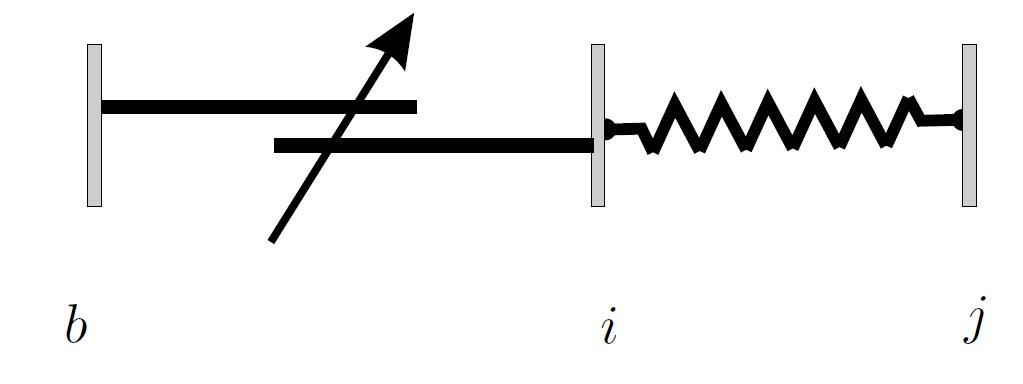
\includegraphics[width=0.55\textwidth]{variablespring.jpg}
	\caption[Variable rest-length spring]{Variable rest-length spring \cite{Stramigioli_99}}
	\label{FIG:variablespring}
\end{figure}
Towards a PHS representation we need to identify the components contributing to the deformation twist of the spring $ T_i^{j} $: the displacement twist of the bodies attached to the spring $T_b^{j} $ and the twist resulting from a commanded change of rest-length $T_i^{b}$ \cite{Stramigioli_01c}.
\begin{equation}
	T_i^{j} = T_b^{j} + Ad_{H_b^j} T_i^{b}
\end{equation}
Since no additional energy storages were introduced, the Hamiltonian function is equal to the case of the previous simple spring. We can write the two-port Hamiltonian system of a variable length spring as
\begin{eqnarray}\label{EQ:variablerestlengthspring}
	\dot{H}_i^j =\left( \begin{pmatrix}1 & Ad_{H_b^j}\end{pmatrix} \begin{pmatrix}T_b^{j} \\ T_i^{b}\end{pmatrix} \right) H_i^j\\
	\begin{pmatrix}W_b^{j,j} \\ W_i^{b,b}\end{pmatrix}  = \left( \begin{pmatrix}1 \\ Ad_{H_b^j}^T\end{pmatrix} \frac{\partial V_{i,j}}{\partial H_i^j} \right) (H_i^j)^T
\end{eqnarray}

\subsubsection{Inertias}
The kinetic energy of a body is a function of its relative motion with respect to an inertial frame $ \Psi_0 $. The body's dynamic properties are described by the inertia matrix $M_b$, which consists of mass and rotational inertia components. Consider the classical description of a body's dynamics:
\begin{equation}
	M_b \dot{T}_b^{b,0}  = C_b T_b^{b,0} + W_b^b
\end{equation}
Where $C_b$ accounts for Coriolis and Centripetal terms and $W_{ext}^b$ is the external wrench acting on the body.\\
Recall from Table \ref{TAB:PHSvar_mechanic} that the energy state variable is the momentum $P_b^b = M_b T_b^{b,0}$ and the flow variable is the wrench, we can reformulate the previous equation to PHS form
\begin{eqnarray}
	\dot{P_b^b} = C_b \frac{\partial V_k(P_b^b)}{\partial P_b^b} + I_6 W_{ext}^b \\
	T_b^{b,0} = I_6 \frac{\partial V_k(P_b^b)}{\partial P_b^b}
\end{eqnarray}
The kinetic energy function is given as $V_k = \frac{1}{2}(P_b^b)^T M_b^{-1} P_b^b$.
In cooperative manipulation we often deal with heavy objects, it is thus inevitable to model gravity of the virtual object.  A potential energy is assigned to a mass in the gravitational field. This can be modelled with a spring connecting the body and an inertial frame associated with the ground. This spring can be formulated as a PHS using the left translation (\ref{EQ:lefttranslation})
\begin{eqnarray}
	\dot{H}_b^0 = H_b^0 T_b^{b,0}\\
	W_b^{b,0} = (H_b^0)^T\frac{\partial V_{g}}{\partial H_b^0}
\end{eqnarray}
Where $V_g$ is the gravitational potential energy of the body. For a combined description the potential and kinetic energy add up: $V_{kg} = V_k + V_g$. Since there are two types of energy stored by \emph{one} body, the twists in both energy systems are equal. The wrenches on the body add up   
\[W_{kg}^b = W_{ext}^b + C_b \frac{\partial V_{kg}}{\partial P_b^b} - (H_b^0)^T \frac{\partial V_{kg}}{\partial H_b^0} \]
Note that the negative sign in the upper equation comes from $W_b^b = - W_b^{b,0} $\\
With this knowledge we can write the combined PHS representation
\begin{eqnarray} \label{EQ:PHSinertia}
\begin{pmatrix}\dot{H}_b^0 \\ \dot{P_b^b}\end{pmatrix} =
\begin{pmatrix} 0 & H_b^0  \\
- (H_b^0)^T & C_b\end{pmatrix}
\begin{pmatrix}\frac{\partial V_{kg}}{\partial H_b^0} \\ \frac{\partial V_{kg}}{\partial P_b^b}\end{pmatrix}+
\begin{pmatrix}0 \\ W_{ext}^b\end{pmatrix} \\
T_b^0 = \begin{pmatrix}0 & Ad_{H_b^0}\end{pmatrix}
\begin{pmatrix}\frac{\partial V_{kg}}{\partial H_b^0} \\ \frac{\partial V_{kg}}{\partial P_b^b}\end{pmatrix}
\end{eqnarray}


\subsubsection{Dampers}
Dampers do not have a state since they do not store energy, they only dissipate it. For sake of completeness note that energy is not "destroyed" in the dampers but transformed in to thermal energy. This can be modelled with a thermal port connected to the environment, since we are only interested in free energy this port is omitted. The easiest way to achieve damping is a linear resistive element $R$, such that the wrench is directly proportional to twist. Consider for example a body's motion with respect to the inertial frame
\begin{equation}
	W_b^b = R T_b^{b,0}
\end{equation}
Or a damper in parallel with spring
\begin{equation}
	W_i^{j,j} = R T_i^{j}
\end{equation}
The dissipated co-energy is $E_d = \frac{1}{2}T^T R T$.

\section{Control of port-Hamiltonian systems}
\subsection{The Intrinsically Passive Controller (IPC)}
The IPC is a control architecture based entirely on physical intuition. The structure can be seen in Fig. \ref{FIG:IPCsprings}, it is exclusively a geometric interconnection of springs, inertias and dampers. The manipulators are connected with spatial springs to the object. The object is modelled by a virtual inertia and its shape is represented by a sphere that does no necessarily coincide with the actual shape. The resulting virtual object is subjected to forces exerted by the manipulator springs and is connected to the environment with another spatial spring. Note that these springs do not exist in reality, they are models to establish compliant behaviour in the controller. The simulated manipulator forces are then applied to the real object, in order to transfer the virtual complaint behaviour to the real world.\\
\begin{figure}
	\centering
	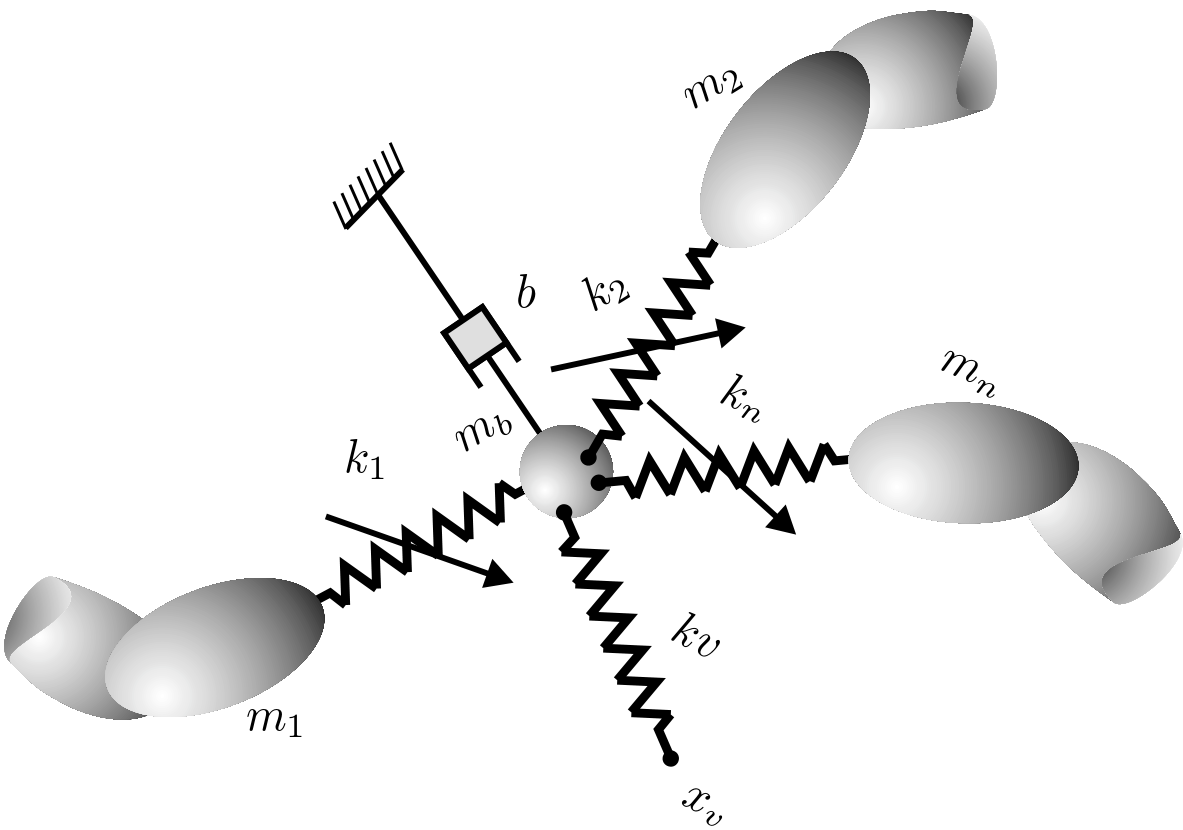
\includegraphics[width=0.8\textwidth]{IPCsprings.png}
	\caption[Structure of the IPC]{Structure of the IPC \cite{Stramigioli_99}}
	\label{FIG:IPCsprings}
\end{figure}
Starting point for the controller design is the virtual object. It is already given by equation (\ref{EQ:PHSinertia}). Springs to environment and manipulator exert wrenches on the object, in terms of port-Hamiltonian representation they are connected through the control port.\\

From a geometric point of view the object-environment spring directly connects to the virtual object frame $\Psi_b$. The other end is attached to the desired object position, denoted with frame $\Psi_v$. This desired object position is the main control objective, by means of this, the motion of the constrained robot-object system is directed. The representation in PHS form is:
\begin{eqnarray}
	\dot{H}_v^b = T_v^{b}H_v^b\\
	W_v^{b,b} = \frac{\partial V_{v,b}}{\partial H_v^b}(H_v^b)^T
\end{eqnarray}
Since we already have a spring relation between the virtual object and the inertial frame it is useful to split this spring into two springs: one between desired position and inertial frame and the other between inertial frame and object position: $H_v^b$ = $H_0^b H_v^0 $.\\
Additionally the have a spring connecting object and each of the $n$-manipulators. As stated before these are variable rest-length springs, to allow for contraction and widening of the formation. Therefore the springs do not connect to the object frame but to a additional supporting frame denoted by $\Psi_v(i)$, which is rigidly attached to $\Psi_b$. Clearly the frames $\Psi_v(i),\; i=1...N$ define the sphere of the virtual object. The springs are situated between the manipulators and the virtual object sphere: $H_{v(i)}^i$ The rest-length is between the sphere and the virtual object frame: $H_b^{v(i)}$, the set-up is illustrated in Fig. \ref{FIG:IPCobject}.
\begin{figure}
	\centering
		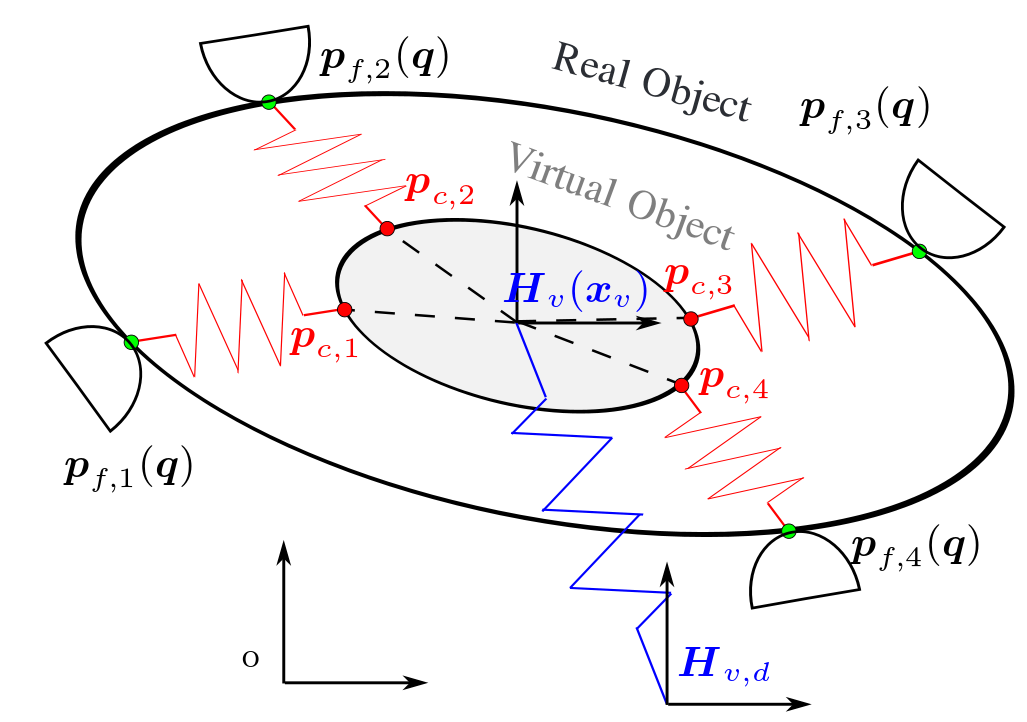
\includegraphics[width=0.8\textwidth]{IPCobjects.png}
		\caption[Virtual object and springs]{Virtual object and springs \cite{Wimboeck_08}}
		\label{FIG:IPCobject}
\end{figure}
 The spring forces act on the virtual object in the virtual contact points $\Psi_{v(i)}$. Therefore we need to map the spring forces to the object. This is done by the grasp map, a well known concept in cooperative manipulation (see e.g. \cite{CoopManipHandbook}). It relates both wrenches and motion between manipulators and object. For example the relation of the $i$-th spring to the object (angular) velocity $(\omega_b^T, v_b^T)^T$ is
\[ \begin{pmatrix}\omega_{v(i)} \\ v_{v(i)}\end{pmatrix} = \begin{pmatrix}\omega_b  \\ v_b + p_{v(i)}^b \times \omega_b \end{pmatrix} \]
We can combine this for all $ n $-manipulators and obtain the grasp matrix
\[ G = \begin{pmatrix*}[l]
S(p_{v(1)}^b) & I_3 \; \cdots \; S(p_{v(N)}^b) & I_3 \\ I_3 & 0_3 \; \cdots \; I_3 & 0_3 \end{pmatrix*} \]
Wherein $S(\cdot)$ denotes the skew symmetric operation, defined in (\ref{EQ:skewsymmetricop}).
The grasp matrix is a useful tool relating both twists and wrenches between object and manipulators:
\begin{equation}
W_b = GW \; , \; T = G^T T_b
\end{equation}
Where $W = (W_{v(1)}^T,...,W_{v(N)}^T)^T$ and $T = (T_{v(1)}^T,...,T_{v(N)}^T)^T$ are the stacked vectors of wrenches and twists respectively.\\
Since we have defined geometric structure of the springs, we can give the PHS representation (see also (\ref{EQ:variablerestlengthspring}))
\begin{eqnarray}\label{EQ:variablerestlengthspring}
	\dot{H}_{v(i)}^i = \left( \begin{pmatrix}1 & Ad_{H_b^i}\end{pmatrix} \begin{pmatrix}T_b^{i} \\ T_{v(i)}^{b}\end{pmatrix} \right) H_{v(i)}^i\\
	\begin{pmatrix}W_b^{i,i} \\ W_{v(i)}^{b,b}\end{pmatrix}  = \left( \begin{pmatrix}1 \\ Ad_{H_b^i}^T\end{pmatrix}  \frac{\partial V_{v(i),i}}{\partial H_{v(i)}^i} \right) (H_{v(i)}^i)^T 
\end{eqnarray}
\subsubsection{Geometric interconnection of springs}
To combine all the presented equations to the full system as shown in Fig. \ref{FIG:IPCsprings}, we express the spring equations with respect to the inertial frame $\Psi_0$.
This is done for the virtual object spring by splitting the twists
\[T_b^v = (Ad_{H_0^v} \;\; -Ad_{H_0^v}) \begin{pmatrix} T_b^0 \\ T_v^0 \end{pmatrix}  \]
and the wrenches which obey the principle of action and reaction. From now on we will express wrenches acting on bodies no more on springs, since this is more convenient when various springs act on a single body. Recall from subsection \ref{[SS:euclideanspacemotions]} that $W_v^b = -W_v^{b,b}$.
\[ \begin{pmatrix}W_b^{0} \\ W_v^{0}\end{pmatrix}  = 
\begin{pmatrix}-Ad_{H_0^v}^T \\ Ad_{H_0^v}^T \end{pmatrix} W_b^{v} \]
We can write the resulting PHS
\begin{eqnarray}
	\dot{H}_b^v = (Ad_{H_0^v} \;\; -Ad_{H_0^v}) \begin{pmatrix} T_b^0 \\ T_v^0 \end{pmatrix} H_b^v \\
	\begin{pmatrix}W_b^{0} \\ W_v^{0}\end{pmatrix}  = 
	\begin{pmatrix}-Ad_{H_0^v}^T \\ Ad_{H_0^v}^T \end{pmatrix}
	\frac{\partial V_{v,b}}{\partial H_b^v} (H_b^v)^T
\end{eqnarray} 
This is done with the manipulator springs in the same manner:
$T_{v(i)}^i = Ad_{H_0^i} T_b^0 - Ad_{H_0^i} T_i^0 + Ad_{H_b^i} T_{v(i)}^b $ Note that the twists and wrenches due to rest-length changes are not brought to the inertial frame, since they represent a distinct power port. As a result we can combine springs in a PHS
\begin{eqnarray}
\underbrace{\begin{pmatrix}\dot{H}_{v(1)}^1 \\ \vdots \\ \dot{H}_{v(N)}^N \\ \dot{H}_b^v \end{pmatrix}}_{\dot{x}_s} =
\begin{pmatrix}
\phi_b & \phi_v & \phi_i & \phi_{rl}\end{pmatrix}
\begin{pmatrix}T_b^0 \\ T_v^0 \\ T_1^0 \\ \vdots \\ T_N^0 \\ T_{v(1)}^b \\ \vdots \\ T_{v(N)}^b\end{pmatrix}
\\
\begin{pmatrix}W_b^0 \\ W_v^0 \\ W_1^0 \\ \vdots \\ W_N^0 \\ W_{v(1)}^b \\ \vdots \\ W_{v(N)}^b\end{pmatrix} = 
\begin{pmatrix} \phi_b^T \\ \phi_v^T \\ \phi_i^T \\ \phi_{rl}^T\end{pmatrix} \frac{\partial V_s}{\partial x_s}
\end{eqnarray}
Where $V_s = V_{v,b} + \sum_{i=1}^N V_{v(i),i} $ is the sum of energy stored in the springs. The geometric interconnection of the springs is described with the matrices $\phi_b , \phi_v , \phi_i , \phi_{rl}$. The relation of the virtual object twist to the relative motion of the springs is 
\[\psi_b = \begin{pmatrix}
\end{pmatrix} \]
\subsubsection{Interconnection of springs and virtual object}
...


This ensures compliant behaviour between object and environment and manipulators and environment. Furthermore object movement is damped with respect to the inertial frame. Dynamic behaviour of the virtual object is simulated in real-time, so no tracking of the object is necessary. The only values that have to be measured are the end-effector positions, the object speed required for the damping term is computed in the simulation. Dampers parallel to the manipulator-object springs are applicable if manipulator speed is measurable.
By varying the rest-length of the manipulator springs a the grasp can be opened or closed. Furthermore in a closed state grasping forces can be specified via the rest-length.


The higher control part has the role of planning and scheduling. It controls the state of energy of the IPC and robot. Trajectory and formation of the manipulators are determined, e.g. moving the robots independently to open or close the grasp, directing the formation of robots to move the object. The grasping process can be controlled by changing the virtual object sphere size. Translation or rotation of the grasped object can be commanded by setting the desired virtual object pose. A human operator taking tasks of the Supervisor causes a delay which can be modelled as transmission line with delay between Supervisor and IPC. The control architecture is still valid in a tele-operation setting. Using scattering the passivity of the IPC can be preserved.
\section{Performance Comparison of control strategies}

To evaluate the presented controllers in an objective way, they are implemented in \emph{Simulink} an compared in terms of:
\begin{itemize}
	\item Trajectory tracking
	\item Dynamic behaviour
	\item Internal Forces
\end{itemize}

%Having explained the problem, and what others have done in similar situations, now explain your approach. Again, give a general overview of your design first, and then go into detail. The important part here is the concept of your work, not the actual implementation! Make sure that the document (particularly a thesis) is self-contained: It should be possible for a reader familiar with the general area to understand your design. Again, be forthright about the limitations of your design. Also, make sure you justify any shortcuts/limitations convincingly.

\subsection{Internal force impedance control with feed-forward of the object dynamics \cite{DePascali_15}}
The set-up consists of four manipulators, distributed symmetrically around the object. In the first case translation in x-direction commanded. Results in Fig. \ref{FIG:abb1} show good tracking behaviour: no position errors in steady state and only small deviations from the desired values during transient phase. No internal stress is exerted on the object. Due to fast translation high manipulator forces occur. 
\begin{figure}[htb]
\centering
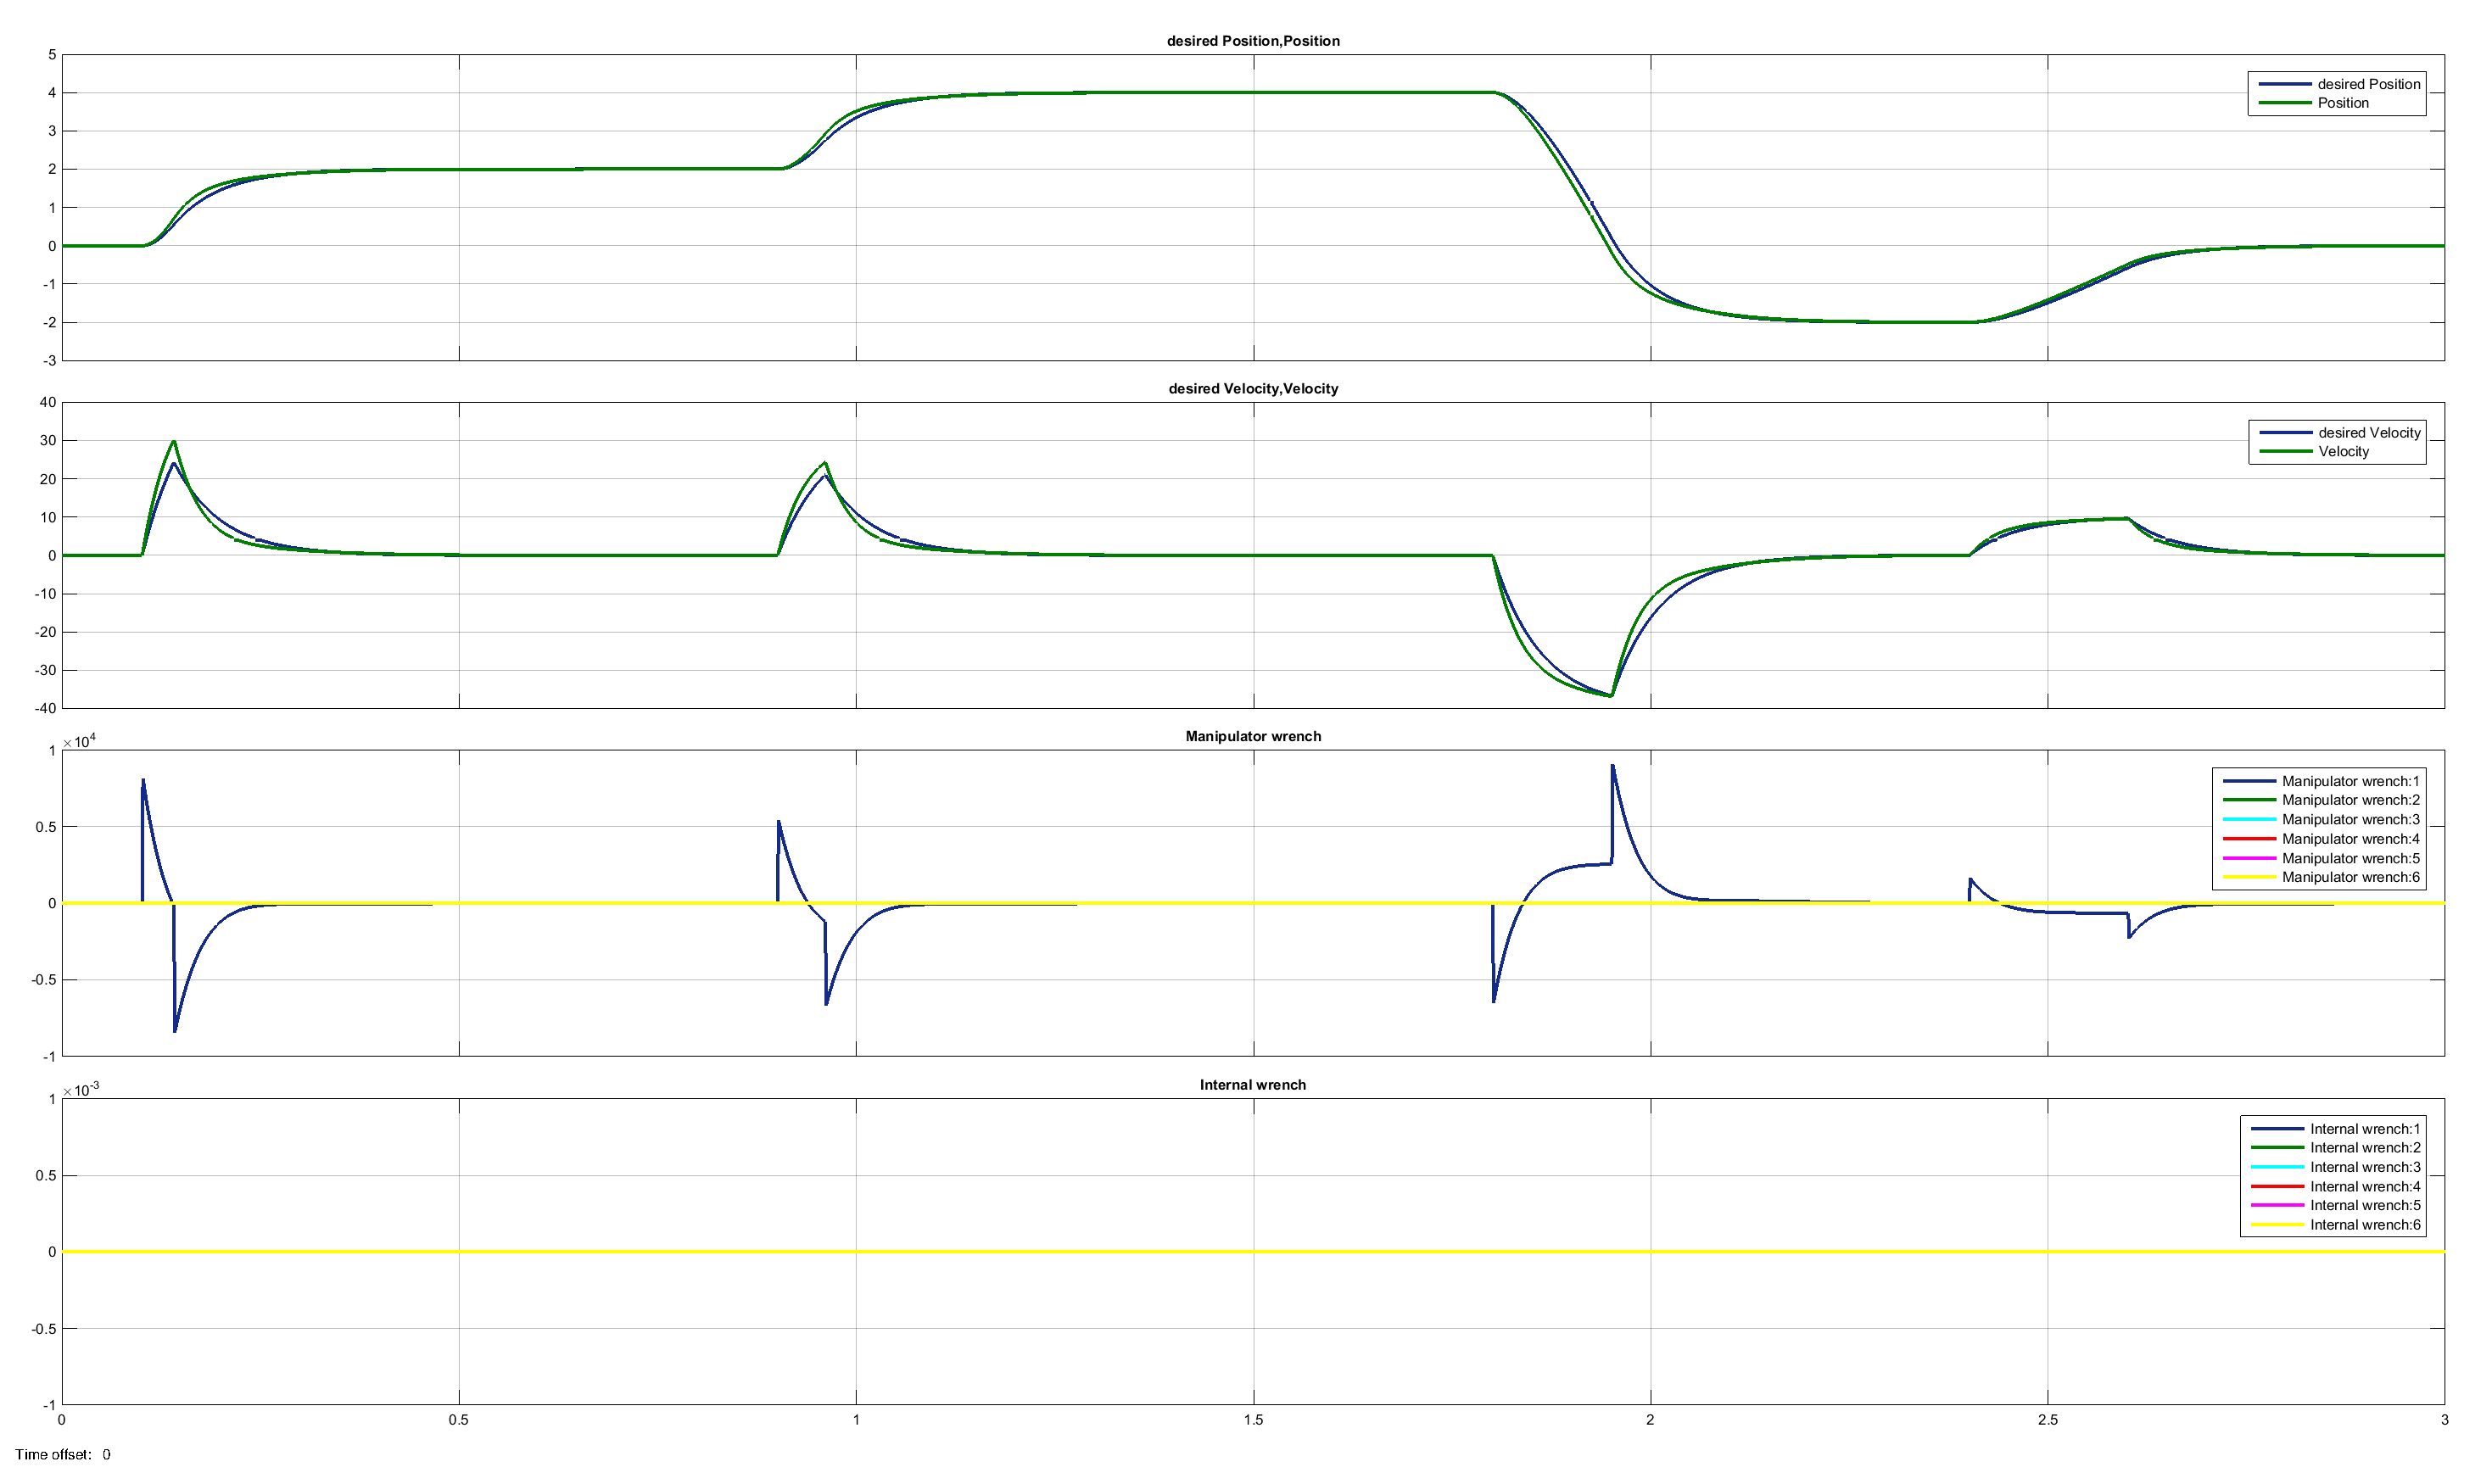
\includegraphics[width=1\textwidth]{Depascliposition.eps}
\caption[Internal force impedance control with feed-forward of the object dynamics: Translation]{Internal force impedance control with feed-forward of the object dynamics: Translation; Graphs from top: Position (desired/actual), Velocity (desired/actual), Force exerted by one manipulator, Internal wrench}
\label{FIG:abb1}
\end{figure}
In the second test case the object is rotated around the $ z $-axis. This is done at a significantly lower speed of at most 1 rad/s, thus the manipulator forces are smaller, desired and actual object trajectory cannot be distinguished in Fig. \ref{FIG:abb2}. However some small internal forces can be seen. Interestingly they are proportional to the simulation step size (running \emph{Simulink's ode3} solver), i.e. a ten-times smaller step size gives ten-times smaller internal forces. Internal forces are calculated based on the geometry of the last simulation step. The correlation between step size and values indicates that these forces are rather due to the discrete nature of the simulation than of the control law generating internal stress. Simulation of the constrained system dynamics as well as calculation of internal wrench is done as described in \cite{Erhart_15/2}.
\begin{figure}[htb]
	\centering
	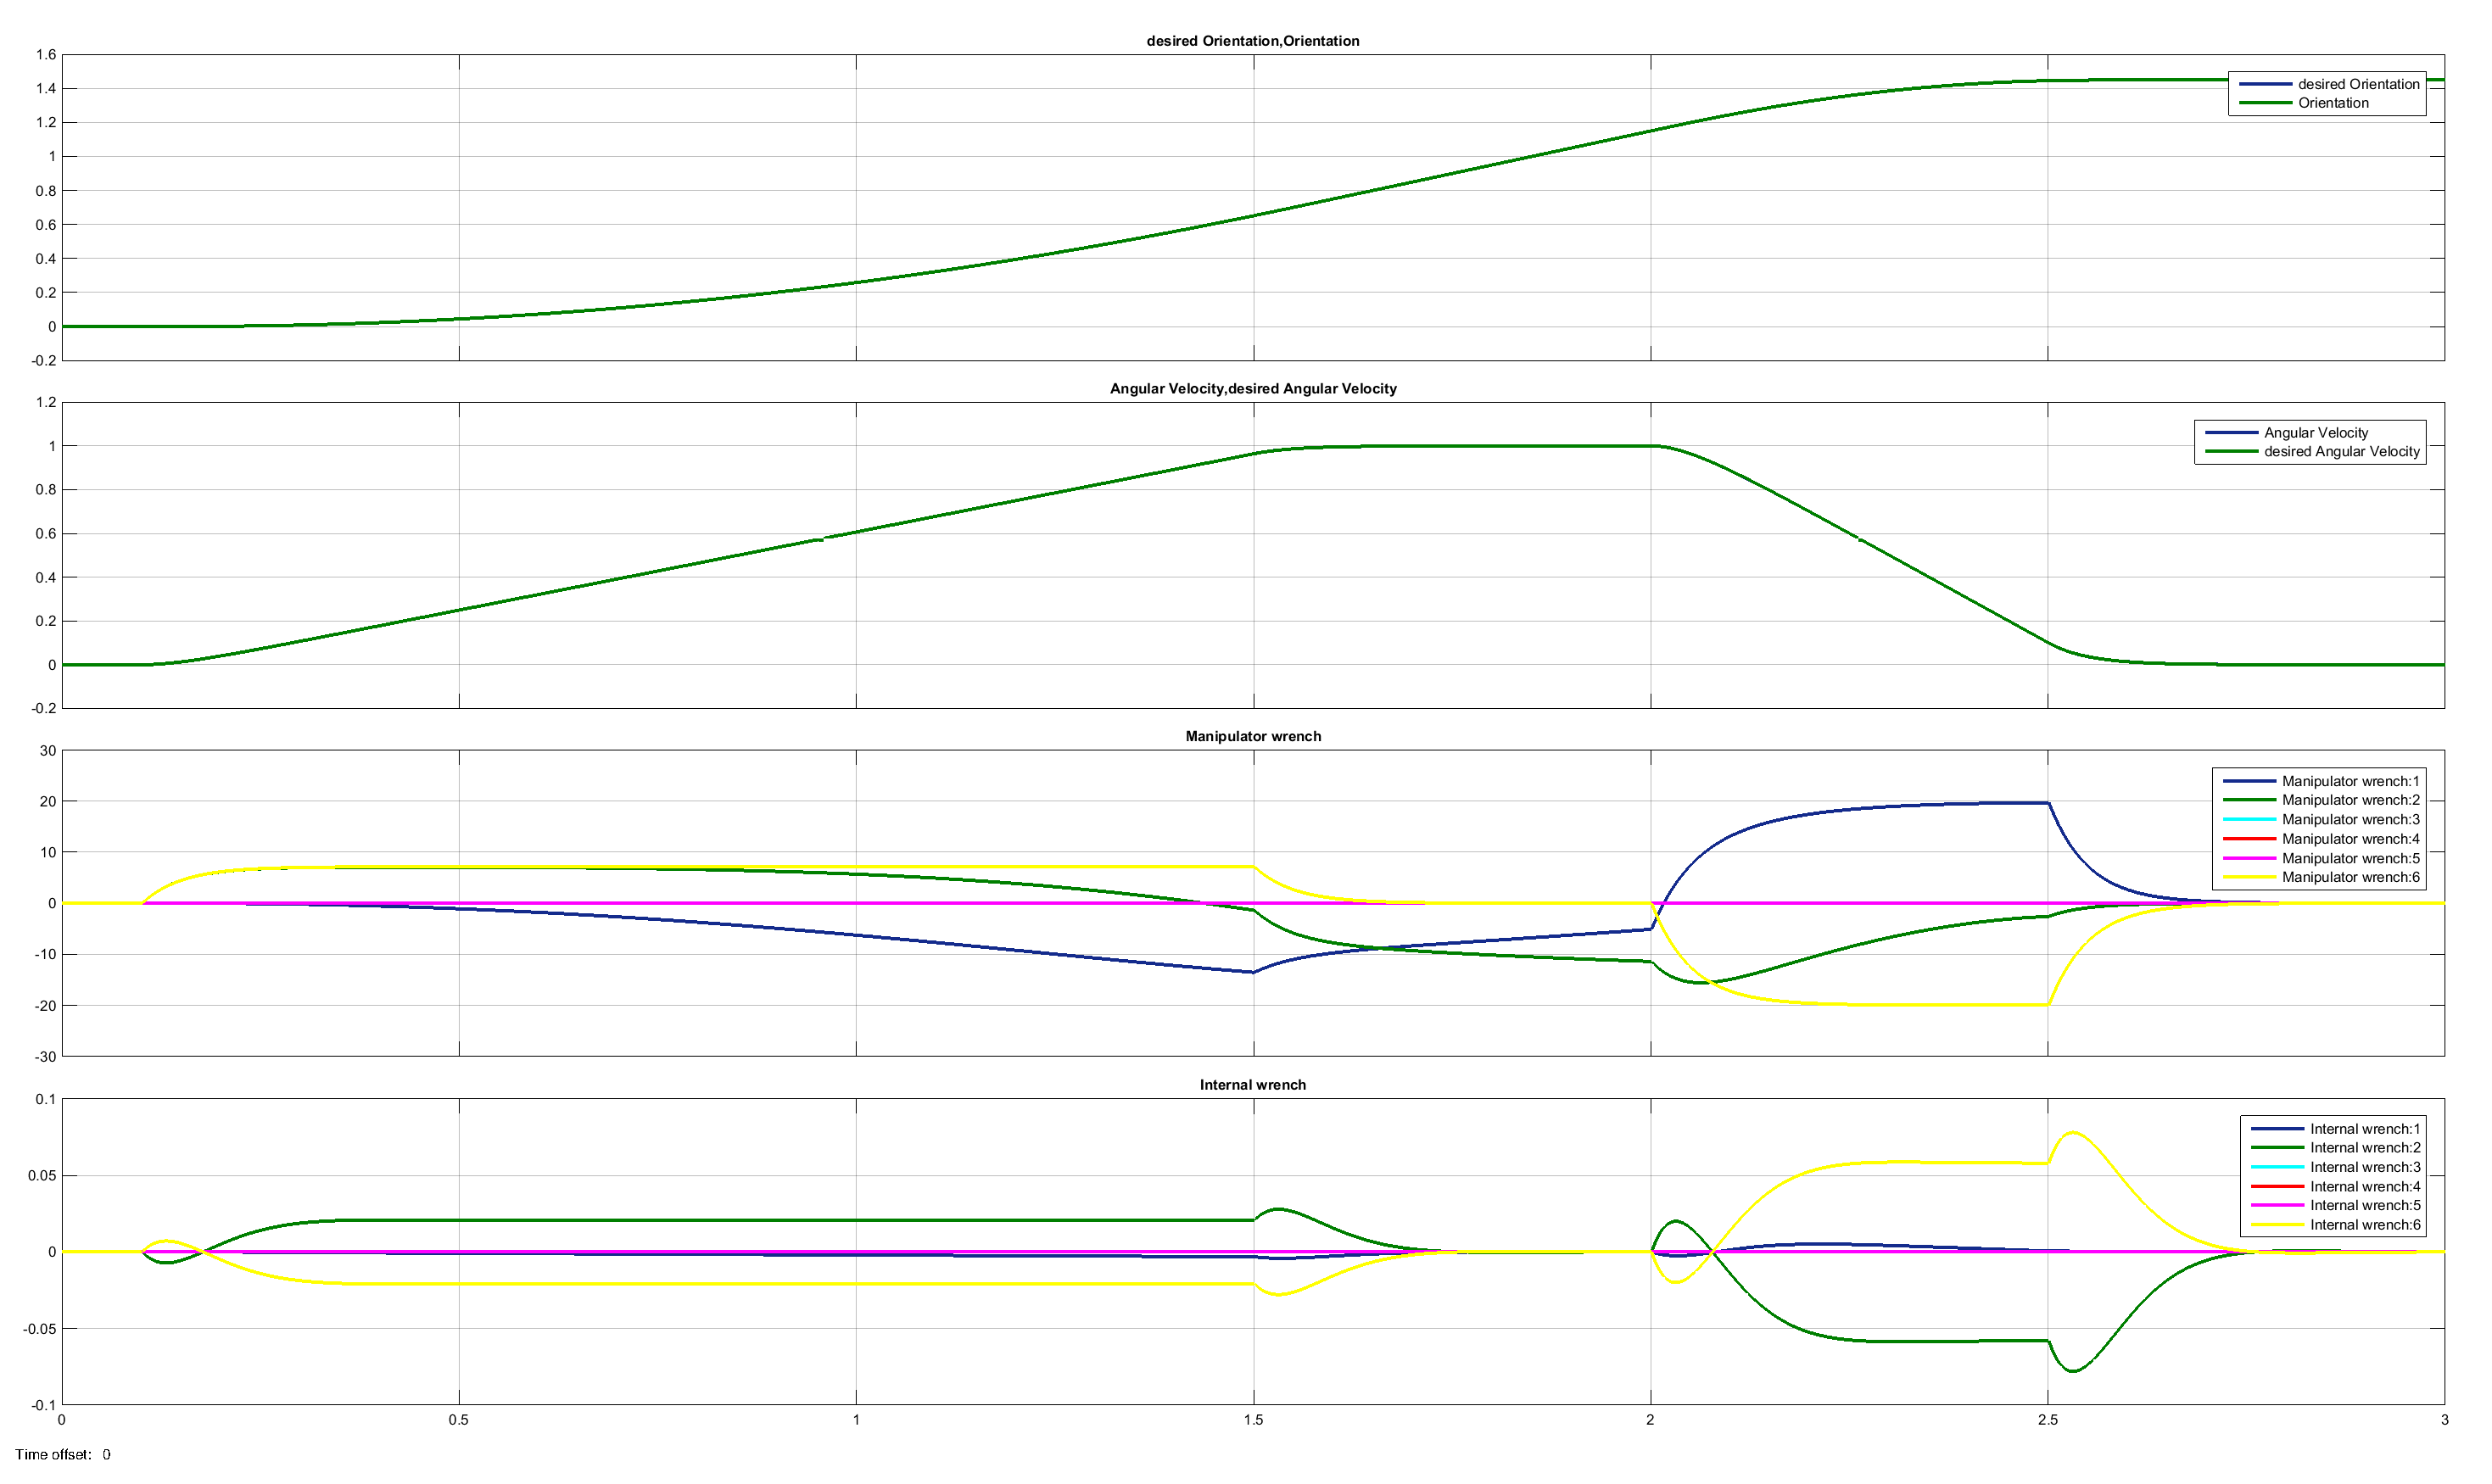
\includegraphics[width=1\textwidth]{Depascaliorientation.eps}
	\caption[Internal force impedance control with feed-forward of the object dynamics: Rotation]{Internal force impedance control with feed-forward of the object dynamics: Rotation; Graphs from top: Orientation (desired/actual), Angular Velocity (desired/actual), Force exerted by one manipulator, Internal wrench}
	\label{FIG:abb2}
\end{figure}


\subsection{Internal and external impedance based reference trajectory generation \cite{Caccavale_01}}
Results for translational motion (see Fig. \ref{FIG:abb3}) are very similar to that of the previous control scheme. When it comes to rotation, higher internal forces can be observed in Fig. \ref{FIG:abb4}. In this case they are not influenced by numerical parameters of the simulation.
This architecture in contrast to the previous makes use of measured contact wrenches. Contact wrench as measured can be obtained from the constrained system simulation. As described in subsection \ref{SS:rigidcontrolschemes} this wrench is than decomposed by kineostatic filters in internal and external components. This does not cancel out undesired internal stress but magnifies it: when the contact wrench is not fed back and set to zero in the internal force impedance controller, results are slightly better. Note that the simulation represents an ideal case, where all parameters are exactly known and no deviations in grasp positions occur. Behaviour in a real experiment may be different and this observation does not mean that the kineostatic-filtered feed-back of contact wrench is unjustified in general.
\begin{figure}[htb]
\centering
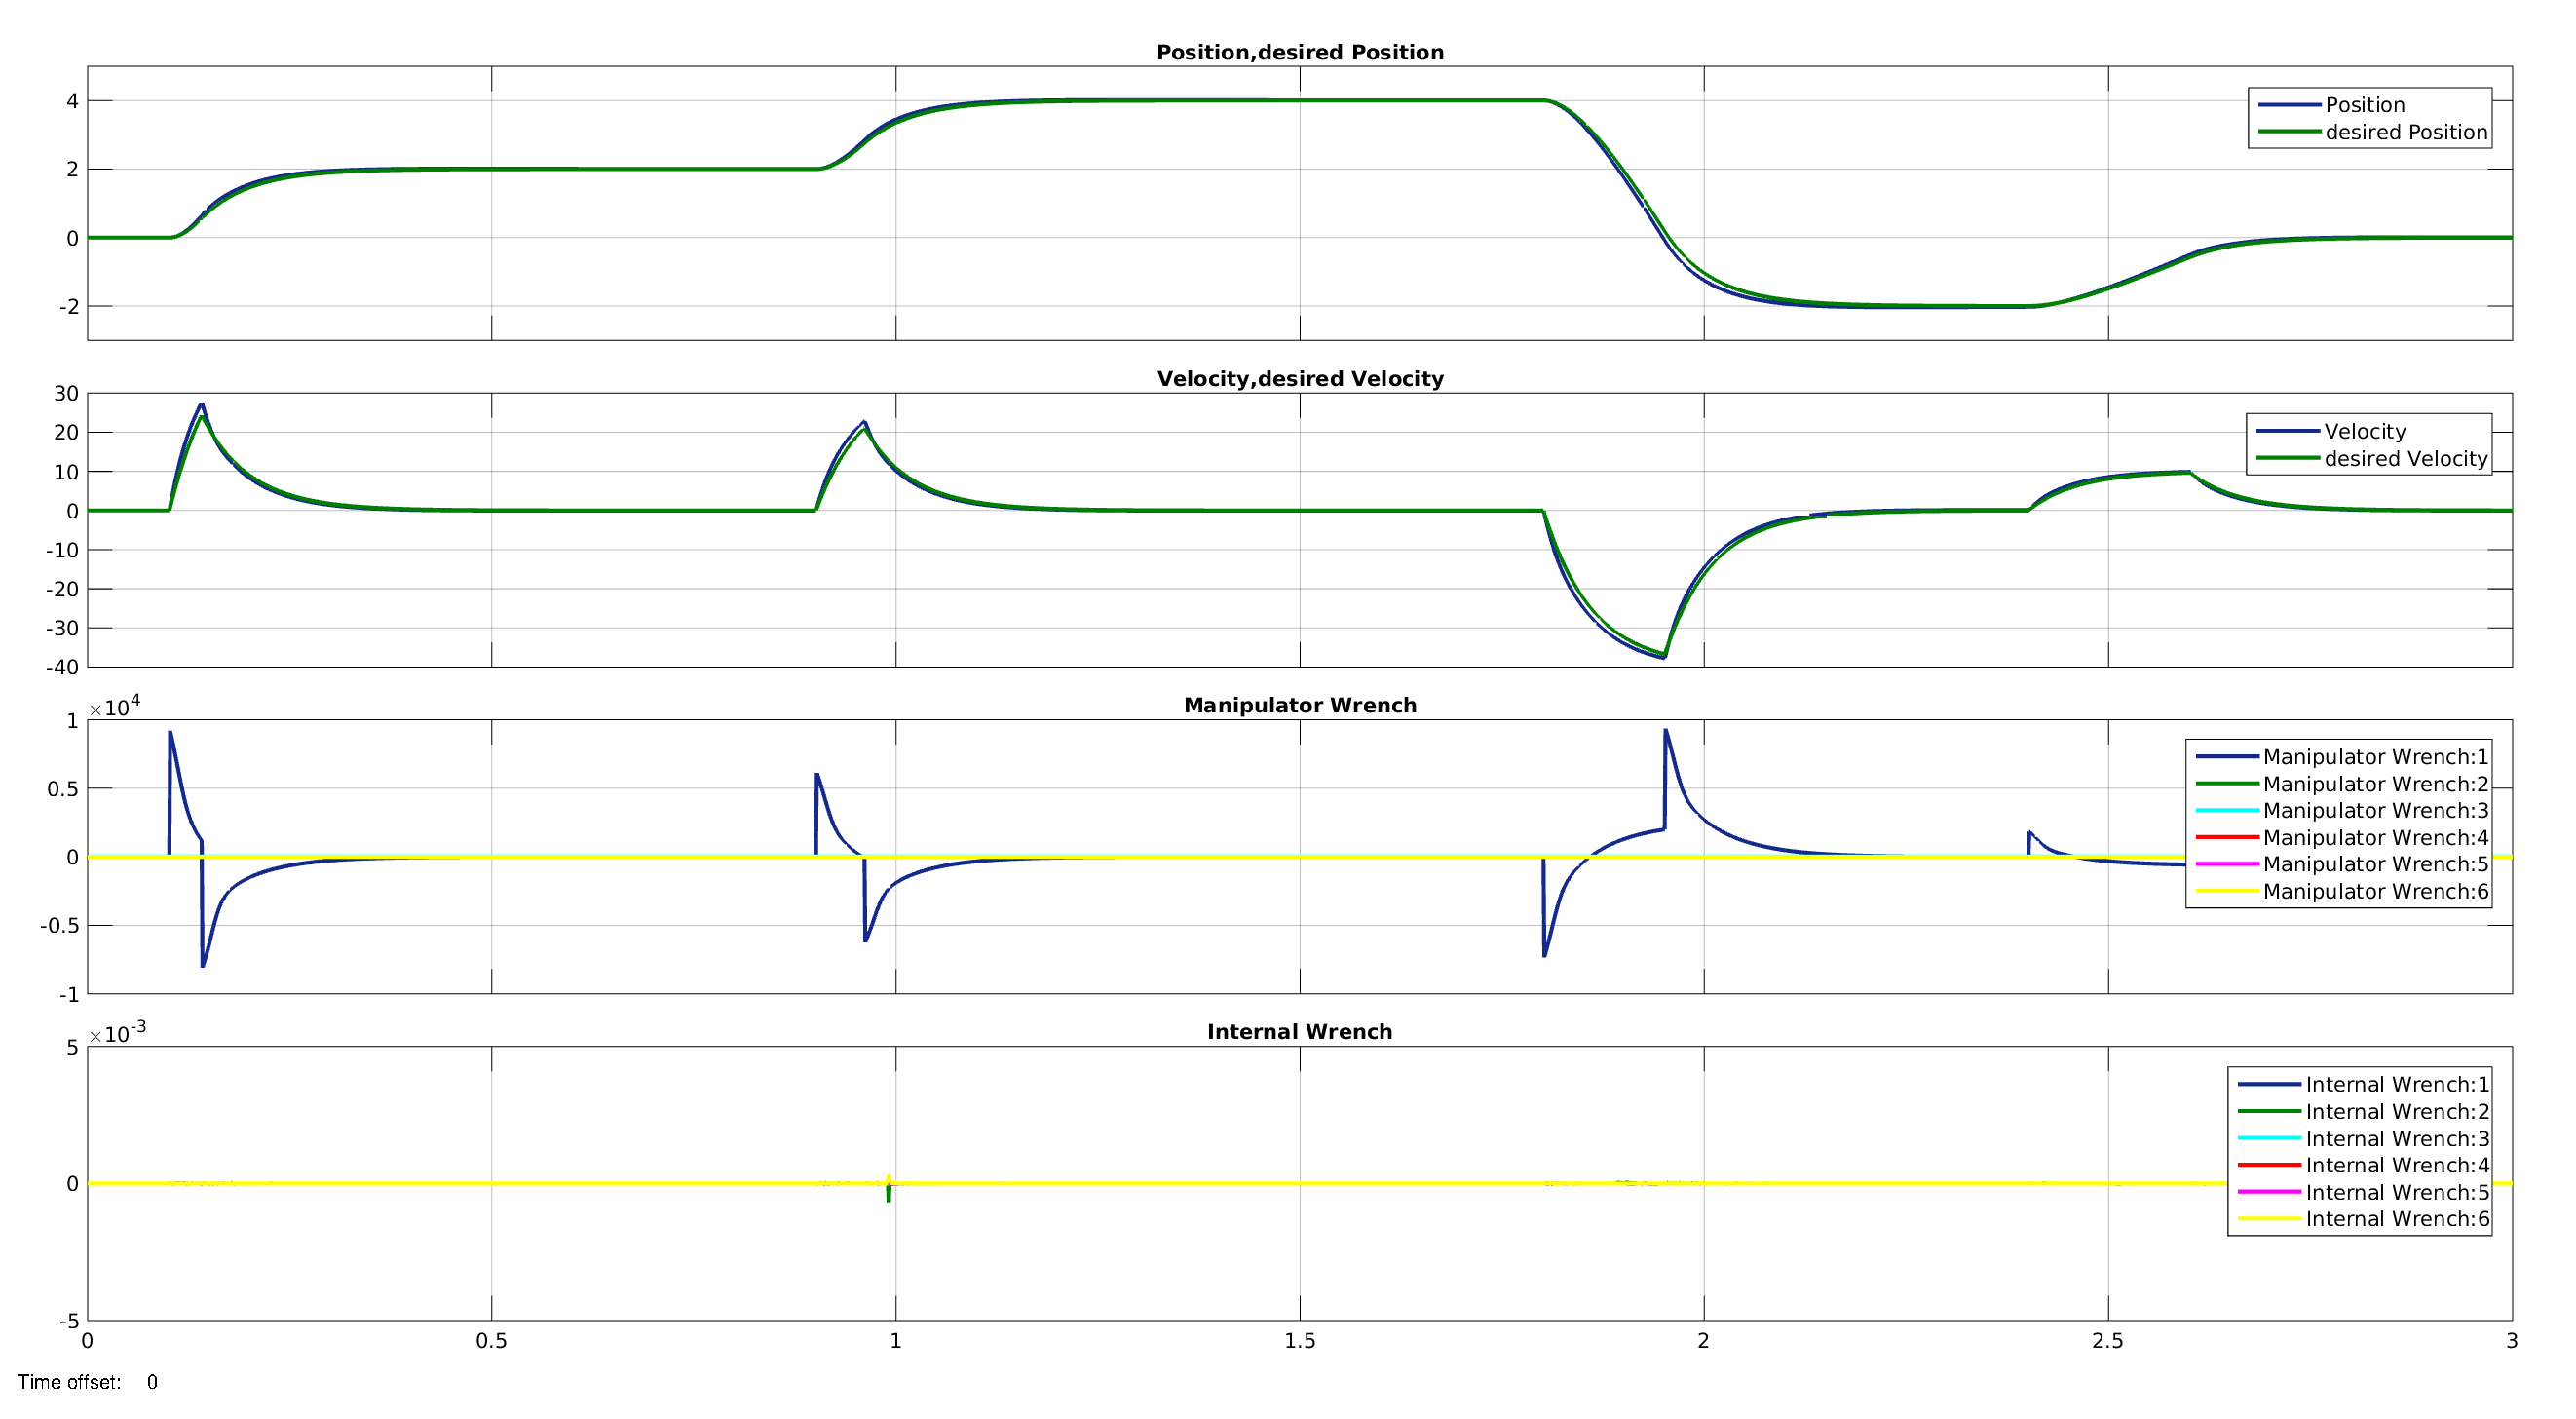
\includegraphics[width=1\textwidth]{Caccavaleposition.eps}
\caption[Internal and external impedance based reference trajectory generation: Translation]{Internal and external impedance based reference trajectory generation: Translation; Graphs from top: Position (desired/actual), Velocity (desired/actual), Force exerted by one manipulator, Internal wrench}
\label{FIG:abb3}
\end{figure}
\begin{figure}[htb]
\centering
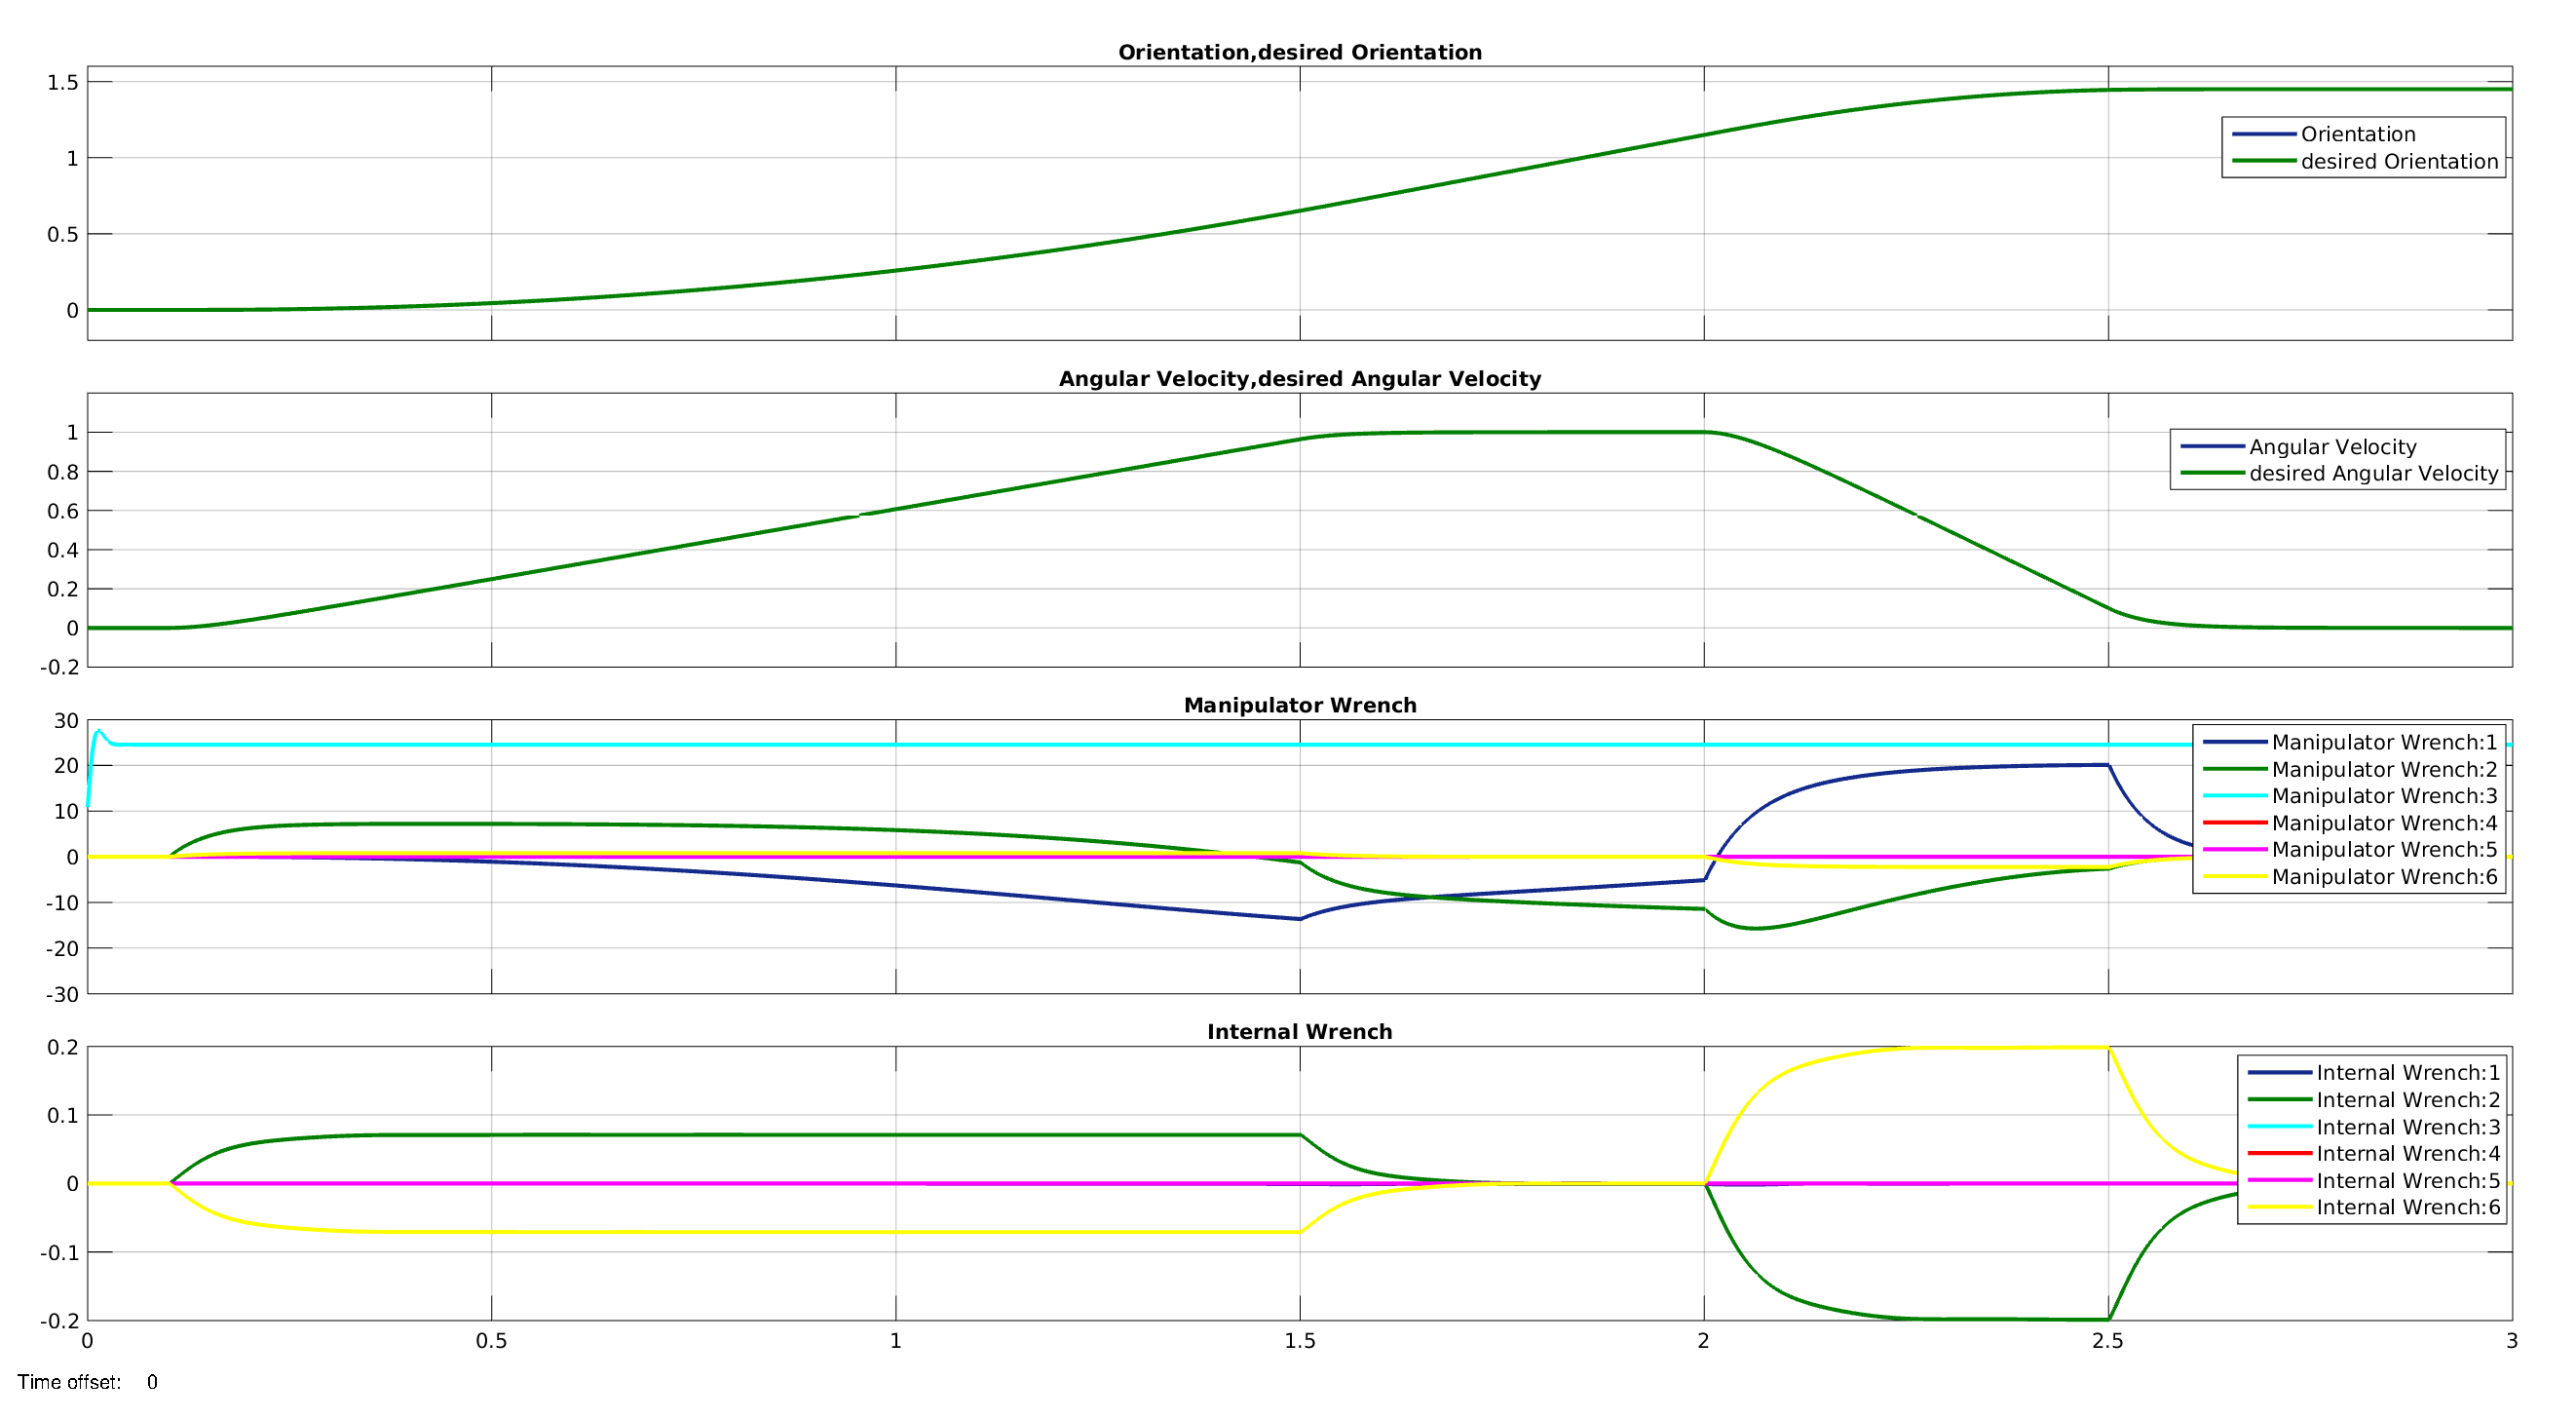
\includegraphics[width=1\textwidth]{Caccavaleorientation.eps}
\caption[Internal and external impedance based reference trajectory generation: Rotation]{Internal and external impedance based reference trajectory generation: Rotation; Graphs from top: Orientation (desired/actual), Angular Velocity (desired/actual), Force exerted by one manipulator, Internal wrench}
\label{FIG:abb4}
\end{figure}

%\subsection{Dynamic Intrinsically Passive Controller (IPC) \cite{Wimboeck_08} }
%\section{Implementation}
%
%
%In many (not all cases) there is a clear difference between the general approach (design) and its implementation in your particular circumstances. The design may be more general than what you can do given time and resources. Or you have developed a general design, and are now implementing a prototype on particular hardware. Give all required details. It should be possible to understand all this without referring to the source code. 
%
%This will, in general, include extracts of actual algorithms and hardware components used. Don't list pages of C code, an electronic copy of the source will accompany the submission and should be available to the marker, so there's no point in killing extra trees to put it into the report. Source code, if included at all, goes into the appendix and not the main document.
%
%Make sure you describe your implementation in enough detail. Someone who has nothing else but your thesis report to go by should be able to repeat your work, and arrive at essentially the same implementation. Reproducibility is an important component of scientific work. Also, clearly state the limitations of your implementation, and justify them.
%
%\section{Experimental Results}
%
%A thesis almost always has an experimental part, typically some comparison to other approaches. Benchmarking takes time, for running the experiments, but also for thinking them up in the first place, and for analysing the results. Plan accordingly to spend enough time here!
%
%Think about what makes sense to measure, what you want to learn from your measurements. Think about what is really the relevant contribution of your thesis, and how you can prove that you have achieved your goals. Think about what you can measure in order to get a good insight into the performance of various aspects of your design, how you can distinguish between systematic and accidental effects, how you can convince yourself that your results are right. If you get surprising results, don't just say "surprise, surprise, performance isn't as good as hoped". Find out why. Surprises without explanation indicate either that you are clueless about what's going on, or that you have made a mistake. Unconvincing results, therefore, tend to imply unconvincing marks. 
%
%\paragraph{Statistics:} Measurements always have statistical (sampling) errors. Owing to the deterministic nature of simulations these are sometimes very small, as disturbing factors can be designed. However, the reader should be given an indication of how statistically significant the results are. This is done by providing at least a standard deviation in addition to averages. Whenever the results of several runs are averaged, a standard deviation can (and must) be supplied. After all, you average to reduce statistical errors.
%
%The reproducibility argument applies here just as much as for the implementation. Give enough detail on what you measure, and how you measure it, so that someone who has your implementation (but not your test code) or has re-done your implementation independently, should be able to repeat your measurements and arrive at essentially the same results. In some cases, results seem outright wrong in a thesis. In those cases, not enough detail is provided to allow the supervisor/reader to pinpoint the likely source of the error. Often the cause is systematic errors resulting from an incorrect measurement technique. If it seems wrong, and the text doesn't convince the reader that it is not wrong, the reader will assume that it is wrong.
%
%\section{Discussion}
%
%Discuss and explain your results. Show how they support your thesis (or, if they don't, give a convincing explanation). It is important to separate objective facts clearly from their discussion (which is bound to contain subjective opinion). If the reader doesn't understand your results, reconsider if you have managed to extract the core information and explain it in a straightforward way.

%_______________________________________________



%_____Zusammenfassung, Ausblick_________________________________
\chapter{Conclusion}
  

%Don't leave it at the discussion: discuss what you/the reader can learn from the results. Draw some real conclusions. Separate discussion/interpretation of the results clearly from the conclusions you draw from them. (So-called "conclusion creep" tends to upset reviewers. It means surrendering your scientific objectivity.) Identify all shortcomings/limitations of your work, and discuss how they could be fixed ("future work"). It is not a sign of weakness of your work, if you clearly analyse and state the limitations. Informed readers will notice them anyway and draw their own conclusions, if not addressed properly.
%
%\vspace{\baselineskip}
%Recap: don't stick to this structure at all cost. Also, remember that the thesis must be:
%
%\begin{itemize}
%	\item honest, stating clearly all limitations;
%	\item self--contained, don't write just for the locals, don't assume that the reader has read the same literature as you, don't let the reader work out the details for themselves.
%\end{itemize}
%
%
%
%This chapter is followed by the list of figures and the bibliography. If you are using acronyms, listing them (with the expanded full name) before the bibliography is also a good idea. The acronyms package helps with consistency and an automatic listing.


%_______________________________________________________________


%_____Abbildungsverzeichnis_________________________________
\cleardoublepage
\addcontentsline{toc}{chapter}{List of Figures} 
\listoffigures 	 %Abbildungsverzeichnis

%___________________________________________________________

%_____Literaturverzeichnis_________________________________
\cleardoublepage
\addcontentsline{toc}{chapter}{Bibliography}
\bibliography{mybib}{}
\bibliographystyle{alphaurl}
%__________________________________________________________


%_____License_________________________________
\cleardoublepage
\chapter*{License}
\markright{LICENSE}
This work is licensed under the Creative Commons Attribution 3.0 Germany
License. To view a copy of this license,
visit \href{http://creativecommons.org/licenses/by/3.0/de/}{http://creativecommons.org} or send a letter
to Creative Commons, 171 Second Street, Suite 300, San
Francisco, California 94105, USA.
%__________________________________________________________

\end{document}
